%------------------------------------------------------------------------------
% Template file for the submission of papers to IUCr journals in LaTeX2e
% using the iucr document class
% Copyright 1999-2013 International Union of Crystallography
% Version 1.6 (28 March 2013)
%------------------------------------------------------------------------------

%\documentclass[preprint]{iucr}              % DO NOT DELETE THIS LINE
\documentclass{iucr}              % DO NOT DELETE THIS LINE

\usepackage{siunitx}
\usepackage{color}
\usepackage{amsmath,amssymb}
\usepackage{mathtools}


\newcommand{\todo}[1]{{\color{red}[TODO: "#1'']}}
\newcommand{\inblue}[1]{{\color{blue}#1}}
\newcommand{\inred}[1]{{\color{red}#1}}
\newcommand{\ingreen}[1]{{\color{green}#1}}


     %-------------------------------------------------------------------------
     % Information about journal to which submitted
     %-------------------------------------------------------------------------
     \journalcode{S}              % Indicate the journal to which submitted
                                  %   A - Acta Crystallographica Section A
                                  %   B - Acta Crystallographica Section B
                                  %   C - Acta Crystallographica Section C
                                  %   D - Acta Crystallographica Section D
                                  %   E - Acta Crystallographica Section E
                                  %   F - Acta Crystallographica Section F
                                  %   J - Journal of Applied Crystallography
                                  %   M - IUCrJ
                                  %   S - Journal of Synchrotron Radiation

\begin{document}                  % DO NOT DELETE THIS LINE

     %-------------------------------------------------------------------------
     % The introductory (header) part of the paper
     %-------------------------------------------------------------------------

     % The title of the paper. Use \shorttitle to indicate an abbreviated title
     % for use in running heads (you will need to uncomment it).

\title{Pairing transfocators in undulator beamlines for low-emittance storage rings}
%\shorttitle{Short Title}

     % Authors' names and addresses. Use \cauthor for the main (contact) author.
     % Use \author for all other authors. Use \aff for authors' affiliations.
     % Use lower-case letters in square brackets to link authors to their
     % affiliations; if there is only one affiliation address, remove the [a].

\cauthor[a]{Manuel}{Sanchez del Rio}{srio@esrf.eu}{address if different from \aff}
\author[a]{Marco}{Cammarata}
\author[a]{Rafael}{Celestre}
\author[a]{Juan}{Reyes-Herrera}

\aff[a]{European Synchrotron Radiation Facility, 71 Avenue des Martyrs, 38000 Grenoble \country{France}}
% \aff[b]{Second affiliation address}

     % Use \shortauthor to indicate an abbreviated author list for use in
     % running heads (you will need to uncomment it).

%\shortauthor{Soape, Author and Doe}

     % Use \vita if required to give biographical details (for authors of
     % invited review papers only). Uncomment it.

%\vita{Author's biography}

     % Keywords (required for Journal of Synchrotron Radiation only)
     % Use the \keyword macro for each word or phrase, e.g. 
     % \keyword{X-ray diffraction}\keyword{muscle}

%\keyword{infrared beamline}

     % PDB and NDB reference codes for structures referenced in the article and
     % deposited with the Protein Data Bank and Nucleic Acids Database (Acta
     % Crystallographica Section D). Repeat for each separate structure e.g
     % \PDBref[dethiobiotin synthetase]{1byi} \NDBref[d(G$_4$CGC$_4$)]{ad0002}

%\PDBref[optional name]{refcode}
%\NDBref[optional name]{refcode}

\maketitle                        % DO NOT DELETE THIS LINE

\begin{synopsis}
xxx
\end{synopsis}

\begin{abstract}
Abstract goes here.
\end{abstract}


     %-------------------------------------------------------------------------
     % The main body of the paper
     %-------------------------------------------------------------------------
     % Now enter the text of the document in multiple \section's, \subsection's
     % and \subsubsection's as required.

\section{Introduction}

\todo{too much lens oriented.. turn it to partial coherence...}

After the first experimental demonstration of the feasibility of using lenses to focus synchrotron X-ray beams \cite{Snigirev1996}, an exceptional development has been produced in the field. It concerns the material used (typically Be, Al, and C$^*$), the surface shaping methods (punched lenses \cite{XX}, lithographic techniques \cite{XX}), reducing of the surface errors (shape, waviness and roughness), and different techniques for piling lenses. Single lenses with a shape designed to minimize (e.g., parabolic \cite{XX}) or completely reduce optical aberrations (ellipses \cite{XX}, cartesian ovals \cite{XX}) can be used for micro- and nano-focusing \cite{XX} applications. A Compound Refractive Lense (CRL) is a pile of single lenses allowing shorting the focal length. There are typically used to focus or collimate the beam, but they can also perform as monochromators in combination with an slit that select a photon energy bandwidth exploiting the energy-dispersion (chromatic aberration) of the light refraction. A transfocator is a pile of CRLs with possibility of switching on and off the individual CRLs, thus providing an almost continuous variation of the focal distance. 

A lens system for X-ray beamline applications is usually described by parameters related to the lens focal $F$ (typically the curvature $R$ and refraction index $n=1-\delta+i\beta$) which can be approximated by the equation
\begin{equation}
    \label{eq:F}
    F=\frac{R}{2 N \delta},
\end{equation}
and the lens absorption, which depends on $\beta$ and is used to define a variety of parameters such as the effective aperture \cite{XX}, and gain \cite{XX}. For multiple lenses (CRLs or transfocators), the global focal distance is $F^{-1}=F_1^{-1}+F_2^{-1}+...$. 

For synchrotron beamlines, we are interested in the position of the focal spot and the ``size" of the focal spot. If the source is placed at a distance $p$ from the lens, applying geometrical optics, the beam refracted by the lens has its waist at a distance $q$ given by the lens equation
\begin{equation}
    \label{eq:lens}
    \frac{1}{f} = \frac{1}{p} + \frac{1}{q},
\end{equation}
therefore $q=F p / (p-f)$. The system has a magnification $M=q/p$, so for a source of size $s$ the image at the waist has a lateral dimension of $Ms$. 

This last result, which is well known by beamline designers, operators and users, is valid using incoherent beams, or coherent beams with large numerical aperture (NA). In the case of coherent beams with reduced numerical apertures, it has been shown that the focal position ``moves" towards the lens position when NA reduces (see e.g., \cite{Tanaka:85}, and references therein). As far as the author's knowledge, this effect has never been studied in the context of X-ray beams. 

In this paper we study the focal parameters (position, size, intensity) given by a partial coherent beam, where the NA and coherence fraction are controlled by an aperture. We analyze the focal position originated by a compound system of two lenses, CRLs or transfocators. For this analysis, we have developed an innovative algorithm for fully describing partial coherence from undulator beams using coherent mode decomposition. This method is based on the separated analysis of the horizontal and vertical directions (1D model). The results are compared with fully 2D methods (SHADOW hybrid \cite{XX}, SRW \cite{XX}, COMSYL \cite{XX}). We apply the results to the study of a two transfocator system that is being designed for the new ID18 beamline at the upgraded EBS-ESRF \cite{XX}.  
Pairing two transfocators permits to create a focal spot with size that can adapt to the sample dimensions. The transfocators are design to focus the beam to a spot of variable size in a given interval for a large photon energy range. 


\section{A model for simulating an undulator beamline with transfocators}

For the calculations presented in this paper we have developed a new tool for dealing with partially coherence beams produced by undulators in low-emittance storage rings. For that, we developed a 1D model0 of the coherent mode decomposition previously developed in 2D \cite{XX}. The motivation for developing these new tools is to perform quick calculations (e.g., being able to perform parametric calculations in a laptop) with high accuracy in the simulation of the source and beam propagation. We believe that the separation of the real 2D wavefront in two separated 1D wavefronts is well justified for most synchrotron beamlines, where the cross-talk between these two directions is small. This is justified by comparing results with more CPU demanding 1D simulations. The tools developed here are included in the OASYS toolbox \cite{XX}, available in the WOFRY add-on \cite{XX}. These tools are completely scriptable so they can be used from the OASYS interface, which also creates scripts that can be a posteriori modified for batch runs. 
 

\subsection{Wavefront creation and propagation}

In the limiting case of zero emittance (i.e., ``single-electron" or filament beam), the undulator emission is fully coherent and the wavefront can be calculated using the classical electrodynamics \cite{XX}. These equations are implemented in the pySRU python library \cite{XX} that is used to calculate the undulator emission at a given distance from the source. 

The wavefront evolves when transported in free space from two different positions along the optical axis. We used integral propagators to calculate the wavefront in a given point using the wavefront in another position. In wofry we implemented two propagators, obne based on the direct implementation of the  Rayleigh-Sommerfeld integral, and a second one, the zoom propagator, is a Fresnel propagator using FFT. Both propagators are described in \cite{XX}.


\subsection{Wavefront modification by apertures and lenses}

A generic aperture is a mask that transmits a part of the wavefront in a range $[x_{min},x_{max}]$ and absorbs the rest. It can be
\begin{equation}
R(x;\omega) =
\left\{
\begin{matrix}
A,  & \mbox{~~if~~} x_{min} \le x \le x_{max}
\\ 
1 - A, & \mbox{~~elsewhere}
\end{matrix}
\right.
\end{equation}
When the element is a slit, then $A=1$. If it is a beamstop, then $A=0$. If we deal with an optical element of finite length $L$ placed at a grazing incidence angle $\theta$, it acts as a slit of aperture equal the projection of the length on the $x$ axis: $A=1$, $x_{min}=-(L/2) \sin \theta$ and $x_{max}=(L/2) \sin \theta$. 

We can define an ideal lens as a focusing device that converts a plane wave into a spherical wave collapsing to the focus at a distance $f$ from the ideal lens position. Therefore
\begin{equation}
    R(x;\omega) = e^{-i k~x^2/(2 f)}
\end{equation}

\subsubsection{Wavefront modification by a CRLs and transfocators}

\subsubsection{Wavefront modification by a refractive corrector}

...They can also be used to obtain the best surface to focus in a given point. Therefore it is a way to calculate the optimum lens needed.  

\subsection{Partial coherence modeling the undulator beam using coherent mode decomposition}

The electrons in an storage ring are statistically distributed, following (in good approximation) a Gaussian distribution in a 6-dimensional space (three spatial coordinates, two angles to define direction, and the electron energy). Many electrons therefore contribute to photon beam radiation, each one creating a wavefront. The consequence is that the overall radiation cannot be described deterministically which implies that statistical methods are needed, like for describing the electron beam. This is the origin of partial coherence of the synchrotron emission. As stated before, in an ideal storage ring of zero emittance, the electrons follow a filament beam so the emission is fully coherent. As soon as  electron emittance increases, the electrons contributing to the radiation start to have different initial conditions (in the 6-dimensional space) and the overall emission cannot be describe by a single wavefront, but by statistically distributed wavefronts, described by partial coherent optics.

Under some approximations the radiation is 'wide sense stationary' \cite{mandel_wolf}. These conditions are satisfied for light emitted by storage rings (but not for XFELs) \cite{geloni2008}, and can be summarized in
i) the electron bunch length is long enough,
ii) radiation is monochomatized 'not too much' (like by standard monochromators), and 
iii) the radiation frequency is large enough.
It is in this case all the coherent properties of the radiation can be described using the 'cross spectral density' (CSD), a complex function that measures the correlation of the electric field in two different spatial points at a given radiation frequency. It can be mapped in a $(x,y)$ plane at a third coordinate $z$. At that plane, the CSD depends on 5 variables: 

\begin{equation}
W_{2D}(x_1,y_1,x_2,y_2;\omega) = <E^*(x_1,y_1;\omega) E(x_2,y_2;\omega)>
\label{eq:CSD_1D}
\end{equation}

In the following, we suppose that the CSD is separable in its 1D horizontal $x$ and vertical $y$ coordinates, therefore the $W_{2D}$ becomes a product of two CSD functions $W$ of two variables for a given photon frequency $\omega$:

\begin{equation}
W_{2D}(x_1,y_1,x_2,y_2;\omega) = W(x_1,x_2;\omega) W(y_1,y_2;\omega).
\label{eq:CSD_2D}
\end{equation}
Each $W$ function is treated separately in a similar way affecting the $x$ (horizontal) and $y$ (vertical) coordinate.

From the cross spectral density one can calculate the 'spectral density' (usually simply called 'intensity') $I(x;\omega)=W(x,x,\omega)$, and also the complex degree of (transverse) coherence: 
\begin{equation}
\mu(x_1,x_2;\omega) = \frac{W(x_1,x_2;\omega)}{\sqrt{I(x_1;\omega)}\sqrt{I(x_2;\omega)}}
\label{eq:DTC}
\end{equation}
The modulus of the complex degree of coherence is one for a completely coherent beam and zero for an incoherent beam. 

An important result in partial coherence optics permits to describe the radiation as an infinite sum of independent coherent modes (in the sense of orthonormality) :

\begin{equation}
W(x_1,x_2;\omega) = \sum_{n=0}^{\infty} \lambda_n(\omega) \Phi^*(x_1;\omega) \Phi(x_2;\omega) 
\label{eq:CMD}
\end{equation}
where $\lambda_n$ (eigenvalues) are the intensity weights and the $\Phi$ are the coherent modes (eigenfunctions). 
Some important characteristics of this coherent mode decomposition are: i) the modes are orthonormal (in the integral sense), ii) the modes maximize the spectral density, the first mode is more intense than the second, and so on, meaning that the truncated expansion is optimal, and iii) there is complete coherence if and only if there is only a single mode. If one can truncate the infinite series to a limited number of modes $N$ which contain a good percentage of the spectral density, the numerical storage of the $N$ modes that depend on two spatial variables is usually more economic than the storage of the cross spectral density $W$ that depends on four variables. 
The eigenvalues $\lambda_n$ are a measure of the intensity. One can define the occupation $\eta$ of the i-th mode as the normalized intensity: 

\begin{equation}
\eta_i(\omega) = \frac{\lambda_i(\omega)}{\sum_{n=0}^{\infty} \lambda_n(\omega)}
\end{equation}

From these arguments, it is now natural to rigorously define Coherent Fraction ($CF$) as the occupation of the first coherent mode: $CF=\eta_0$.

The eigenvalues and the coherent modes are the solution of the homogeneous Fredholm integral equation of second kind \cite{XX}.
This is an eigenvalue problem. The numerical solution is obtained from the diagonalization of the CSD, which is a multivariate tensor when sampled at the point coordinates. This diagonalization problem is solved in 2D (i.e., $W_{2D}$ is a function of 4 variables) using complex numerical algorithms implemented in COMSYL. Fortunately, in 1D, the CSD is a function of two variables, represented in a matrix that can be easily diagonalized using standard tools availables in python-numpy. The numerical calculation of $W(x_1,x_2)$ uses Kim's convolution theorem \cite{XX} as explained in \cite{XX}.

The interest of the coherent mode decomposition method is twofold: the possibility to propagate a partial coherent beam along the beamline by just propagating a few modes (less modes for a more coherent beam) which behave like coherent wavefronts, and the use of the coherent fraction to parametrize the beam coherence along the beamline.  

\todo{How to approximate an undulator beam with GSM  Appendix A}


\subsection{Other 2D methods}
\begin{itemize}
    \item {SHADOW-HYBRID}
    \item SRW Multielectron
    \item COMSYL
\end{itemize}

In addition, we also compared the results with a Gaussian Shell-model in 1D, which is the most simplistic approximation among all partial coherent methods used in this work. 

\section{Effect of NA in focal position for a focused coherent beam}

This section idealizes the ``simple" case of focusing a synchrotron beam with a transfocator. In most beamlines the beam coherence fraction is increased by reducing the aperture of an entrance slit. The beam, with high coherence, is affected by diffraction effects mainly produced at the slit aperture but also at the lens (finite dimension and surface errors). The focal position changes, modifying the focusing propertied of the transfocator. 

\subsection{Preliminary works.}

% The case of a Gaussian beam focused by a lens with a physical aperture modifying the numerical aperture has been thoroughly studied (see e.g., \cite{Tanaka:85}, and references therein).
When the beam is cropped by the slit, the beam waist moves to the lens. Closing more the slit implies that the focus will move more and more to the lens itself, which is reached at the limit of zero aperture. The change of the waist position happens when the Fresnel number\footnote{The factor 4 comes because $a$ is the aperture size so we use $a/2$ for the radius. This can be generalized as $N=a^2 p / (4 \lambda (p-p_a)^2)$ when the slit is not at the lens position.} is smaller than one
\begin{equation}
    N = \frac{a^2}{4 p \lambda}  < 1
\end{equation}. 

After \cite{Belland:82}, there are three possible regimes 
\begin{enumerate}
\item when diffraction effects are negligible, the
characteristics of the Gaussian beam are unchanged
behind the aperture ($N>1$),
\item when the Gaussian
beam is weakly diffracted, it looks in the far-field always as a Gaussian beam, with slightly different characteristics ($N_0<N \le 1$),
\item when the diffraction effects are large ($N<N_0$),
the diffracted beam is no longer Gaussian, and the Gaussian Shell-model cannot be applied.
\end{enumerate}

The transition (1) to (2) will move the focus towards the lens. In the more general case where the numerical aperture is reducing by a slit upstream from the lens ( instead of reducing the lens aperture), the focus will shift to the position $q'=f p_a/(p_a-f)$, a position given by the geometrical optics when the source is placed at the slit position.
 
 
 \subsection{Simulations of the change of focal position when reducing the slit opening}
 
Suppose an aperture placed between the source and the lens, at a distance $p_a$ from the lens ($p_a < p$). Following the geometrical optics, the position of the beam waist after the lens unchanged if the aperture changes. Looking at the waist size, when the aperture size $a$ is larger than the source size $a$, the waist size is always $Ms$ but if $a<s$ the aperture obscures part of the source like if it was an ``effective" smaller source. But, as said, the position of the waist is not modified. 

% Let us consider the simplified case of a fully coherent and monochromatic source with photon wavelength $\lambda$. The intensity at the source plane can be modelled by a Gaussian distribution of  root mean square (RMS) $\sigma_s$. A lens is placed at a distance $p$ from the source. An aperture is placed upstream from the lens at a distance $p_a$ from the lens. If the far-field approximation holds, the beam at the slit plane will have a Gaussian intensity distribution with $\sigma_a=(p-p_a) \lambda /(4 \pi  \sigma_s)$. With the slit fully opened, the ideal lens focuses the Gaussian beam into an image whose size $\sigma_i$ and position $q$ are given by the geometrical optics. When the slit is closed, it crops the beam producing diffraction effects that will affect both the position and size of the focus. 

We calculated the beam evolution using wave optics. The source is an undulator with parameters described in Table XX tuned at $E$=7~keV, and we suppose zero emittance (full coherence). An Be lens of radius $R$=\SI{0.2}{\milli\meter} is placed $p=$\SI{65}{\meter}, and a slit of variable aperture $a$ is placed at $p_a$=\SI{29}{\meter} from the lens. The beam at the slit plane has a $FWHM=$\SI{565}{\micro\meter} and the aperture is open at $a = n \times FWHM$ with different values of $n$ covering from fully opening to a very narrow aperture. The refracted beam is analyzed at different positions from the lens by calculating i) the full-width at half-maximum (FWHM) of the intensity distribution, and ii) the on-axis intensity $I_{axis}$. At the focal position, the FWHM should present a minimum and $I_{axis}$ a maximum. 

\begin{figure}
    \centering
    % \includegraphics[width=0.95\textwidth]{figures/oneTFund_400um.eps}
    % \includegraphics[width=0.95\textwidth]{figures/oneTFund_300um.png}  
    \includegraphics[width=0.95\textwidth]{figures/oneTFund_200um.eps}
    %     \includegraphics[width=0.95\textwidth]{figures/oneTFundGSM_200um.eps}
    % \includegraphics[width=0.95\textwidth]{figures/oneTFundHYBRID_200um.eps}
    % \includegraphics[width=0.95\textwidth]{figures/oneTFund_100um.png}

    \caption{Evolution of the size of a coherent undulator beam cropped by a slit and focused by a lens of $R$=~\SI{0.2}{\milli\meter} 
    The plot shows the FWHM of the beam  as a function of the distance from the lens. The aperture is open at $a = n \times a_{FWHM}$ with different values of $n$ (shown in the legend) and $a_{FWHM}$=\SI{565}{\micro\meter} (the beam FWHM at the aperture plane). The focal positions given by geometrical optics are represented for the source placed wither at its real position (yellow vertical line) or at the slit position (blue vertical line).
    The Fresnel number $N$ calculated at the slit plane is also marked in the legend.
    \todo{redo figure with more care with propagators}
    }
    \label{fig:oneTFund}
\end{figure}

Fig.~\ref{fig:oneTFund} shows the evolution of the beam after being focused by the lens. With the open slit the geometrical optics give a focal position $q=$~\SI{18.4168}{\meter} (source at $p$) and $q_a=$~\SI{28.4089}{\meter} (source at slit position, distant $p_a$ from lens). It can be noticed that for $n=$1 (Fresnel number $N=$35) the situation does not change with respect the open slit because the slit crops the beam only. For $n=0.5$ ($N=8.7$, brown line) the FWHM the size waist increases and the depth of focus also increases, manifested in a flat depression. For smaller values of $n$ and $N$ the minumum shifts to higher distances (e.g., $n=0.1$ red line) and becomes less pronounced. For $n$=0.05 (green line), a a small beam size is found again close to the $q_a$ position, but it presents twin minimum due to the effect of the interference fringes in the intensity distribution. Both minima converge to a the $q_a$ position for $n\le$~0.01 (orange line). 

If the lens focal distance is reduced (using lenses with smaller radius, or piling several lenses), the $q$ and $q_a$ positions shift to shorter distances, and  their respective distance reduces. They converge to a single position, the lens focal length, when it is short enough that both source and slit lens can be considered at infinite. 

The dimension of the waist can be calculated using geometrical concepts only for the limiting cases of waist at $q$ and $q_a$. Here, for the waist at $q$, the beam size is the source size times the magnification (distance lens-waist over distance lens-source) and for the waist at $q_a$, the beam size is the slit aperture times the magnification (distance lens-waist over distance slit-lens). This has been verified numerically (not shown). However, for intermediate slit apertures, where the waist position is in between $q$ and $q_a$, the waist size is different to that predicted by geometric optics. Moreover, it interesting to observe that for these intermediate slit apertures that crop the beam, the waist is larger than those found at limiting positions $p$ and $p_a$.

The calculation shown in Figure~\ref{fig:sizes} refers for the zero emittance case (complete coherence, or CF=1). When the EBS emittance values are considered, a coherent mode decomposition of the undulator source is required to include the partial coherent effects. This is done for the horizontal and vertical directions, resulting a CF (at 7 keV) of 0.13 and 0.58, respectively. These values are much higher than for the old ESRF-1 source, but still low for approximating the beam by a coherent source. Therefore, we propagated a number of modes large enough to contain more than 99\% of the source intensity (36 modes in H and 8 in V). The illumination at the entrance slit plane is \SI{610}{\micro\meter} in H times \SI{566}{\micro\meter} in V. The slit aperture is used to tune the coherence of the beam: closing the slit reduces the CF. In the limit (zero aperture) the beam after the slit is fully coherent (CF=1), but obviously with zero intensity. The choice of the right slit aperture comes from a compromise between coherence and flux. The Figure~\ref{fig:oneTFund} shows the CF after of the H and V 1D beams after the slit for different slit apertures. 

\todo{To compare the coherent case with the partial coherent cases (H and V) ...}


\todo{Calculations with HYBRID: It works!}


\begin{figure}
    \centering
    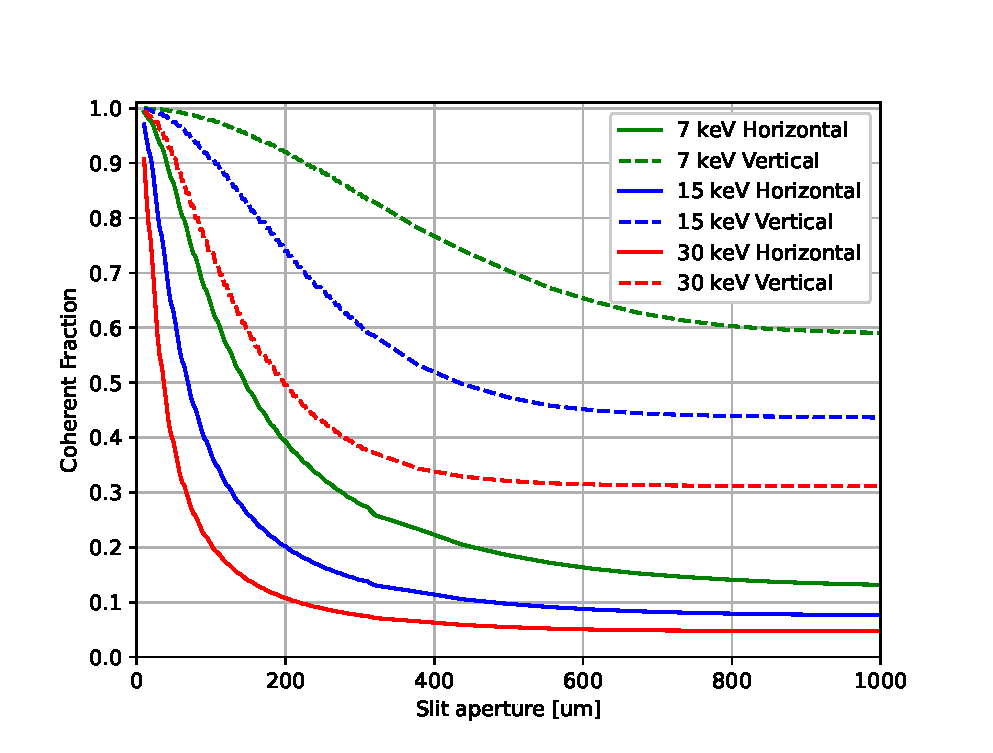
\includegraphics[width=0.95\textwidth]{figures/cf_vs_aperture.eps}

    \caption{
    Coherent fraction in the horizontal and vertical directions as a function of the slit aperture $a$. Top axis shows the $n$ factor as in Fig.~\ref{fig:oneTFund} ($n=565/a$).
    }
    \label{fig:cf_vs_aperture}
\end{figure}





\section{Pairing two transfocators}

%http://lpc1.clpccd.cc.ca.us/lpc/molander/PDFs/Twolenses.pdf

We study here an optical system composed by two lenses (of focal lengths $f_1$ and $f_2$) separated by a distance $D$. Following \cite{Goodman85}, the relationship between object-to-lens-1 distance $p_1$ and the lens-2-to-image distance $q_2$ positions is
\begin{equation}
\label{eq:twolens}
    D-(f_1+f_2)=\frac{f_1^2}{p_1-f_1} + \frac{f_2^2}{q_2-f_2}
\end{equation}

The global magnification is the product of the magnification of the individual lenses. It can be written as

\begin{equation}
\label{eq:magnification}
    M=M_1 M_2=\frac{1-q_2/f_2}{1-p_1/f_1}
\end{equation}

The magnification is not dependent on $D$, however the length of the optical system $L=p_1+D+q_2$ will change if one changes the focal distances of the lenses. For a constant $L$ one can change magnification by changing the inter-lenses distance $D$ (zoom effect). In a synchrotron beamline using transfocators, the magnification can be changes by changing the focal lengths of the transfocators (by adding or removing individual or group of lenses in the transfocator).

We analyze here how to design an optical system using two transfocators and how to set it for the desired magnification. We make a hierarchical anslysis, starting from the most simplified models (geometrical optics), for then using more sophisticated models to include diffraction effects (wave optics) and finally analyse the system illuminated by partial coherent beams.

The system under analysis contains two transfocators, simplified as two lenses of variable focal length. A slit is placed upstream the lens 1. The positions of the elements is determined by room constraints and are considered fixed (although different values could be studied). We study the variation of the spot size as a function of the focal distances. The final goal would be to chose a desired focal size and set the transfocators to obtain it. 

For fixed distances $p_1$, $D$ and $q_2$, we can calculate $f_2$ and magnification $M$ for a given value of $f_1$ (equation~\ref{eq:twolens}). Taking $f_1$ as variable parameter,  Fig.~\ref{fig:f1f2map} shows the maps $f_1$, $f_2$ and $M$.

\begin{table}[]
    \label{table:id18parameters}
    \caption{Caption}
    \centering
    \begin{tabular}{l|c|c}
         element & position [m] & comment\\
         Undulator source& 0 & U20 N=100 K=1.19 (10 keV)\\
         Slit & 35 &
         variable aperture
         %\SI{25}{\micro\meter} H $\times$ \SI{140}{\micro\meter}
         \\
         Transfocator 2D & 65 & 
         collimation optics {\bf CO}
         %$f_H=58.7; f_V=54.3$ 
         \\
         Transfocator 2D & 164 & position 1 {\bf FO1} \\
         Transfocator 2D & 188 & position 2 {\bf FO2}\\
         sample & 200 & focal image {\bf EH2}
    \end{tabular}


\end{table}



For the practical purposes of ID18 (see parameters in Table~\ref{table:id18parameters}), we study two possible positions of lens 2: at \SI{164}{\meter} from the source (initial design, $D$~= \SI{99}{\meter}) and at \SI{188}{\meter} from the source ($D$~= \SI{123}{\meter}). The later implies a shorter, thus cheaper, experimental hutch. Because the effect of shift of focal position due to slit diffraction, discussed before, we consider the two geometrical limiting cases: i) the source at its real position, and ii) the source at the slit position (limit of ``very closed slit"). We expect that the real case will lie in between these two extremes. 

\begin{figure}
    \centering
    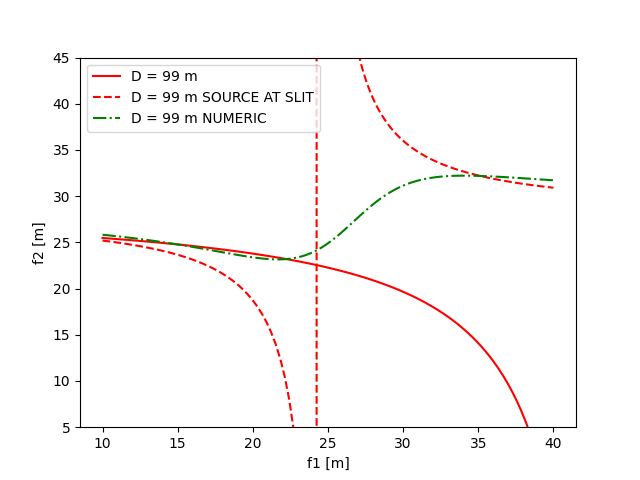
\includegraphics[width=0.95\textwidth]{figures/Figure_trajectories_99.png}
    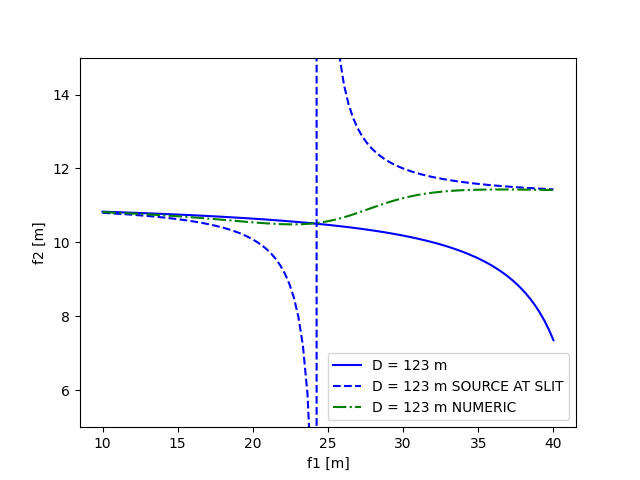
\includegraphics[width=0.95\textwidth]{figures/Figure_trajectories_123.png}
    \caption{Trajectories $(f_1,f_2)$ for $D$~= \SI{99}{\meter} (\inred{top panel}) and $D$~= \SI{123}{\meter} (\inblue{bottom panel}).
    Analytical values are obtained using equation~\ref{eq:lens} with $p_1$~= \SI{65}{\meter} (object at source position) (solid lines) or $p_1$~= \SI{30}{\meter} (object at slit position) (dashed lines). $f_2$ values calculated by a numerical optimization are in \ingreen{green}.
    }
    \label{fig:f1f2map}
\end{figure}

Fig.~\ref{fig:f1f2map} shows the trajectories of $f_2$ as a function of a variable $f_1$. 
The choice of one pair $(f_1,f_2)$ from these curves guarantees that the focus is at the sample position ($L=p_1+D+q_2$~= \SI{200}{\meter} from source). This graphic also shows the value of $f_2$ optimized numerically. They are calculated from the analysis of the wavefront phase impinging on lens 2. A correction profile to focus on the sample is calculated, and from this profile curvature and focal length are deduced. From this graphic it can be observed that the value of $f_2$ obtained numerically goes from the first branch of the analytical values (when the object it at the source position) to  the second branch (when object is at slit), as common sense anticipated.  


Fig.~\ref{fig:magnification} shows the obtained magnification calculated analytically  (equation~\ref{eq:magnification}) and also numerically. The numerical values are calculated in two cases. First with the open slit, a case that would correspond to the analytical case with object at the source position. This is verified in the top panel for $f_1>30$. Second with a slit closed\footnote{All calculations in this section use a Gaussian window to model slit aperture} to $a$~= \SI{25}{\micro\meter} which should approach the analytical results when the object it at the slit position. 
\inblue{A conclusion from this graphic is geometric magnification couls only be used to calculate focal size only in the case of open slit. When the slit crops the beam, numerical calculations are needed.}
\todo{redo these figures and discussion.}



\begin{figure}
    \centering
    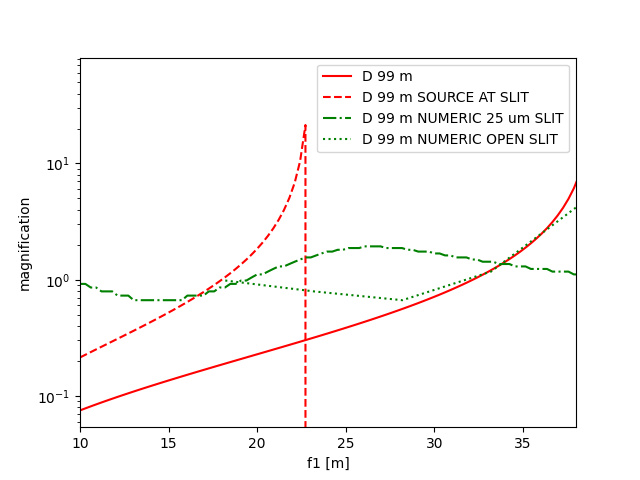
\includegraphics[width=0.95\textwidth]{figures/Figure_magnification_99.png}
    %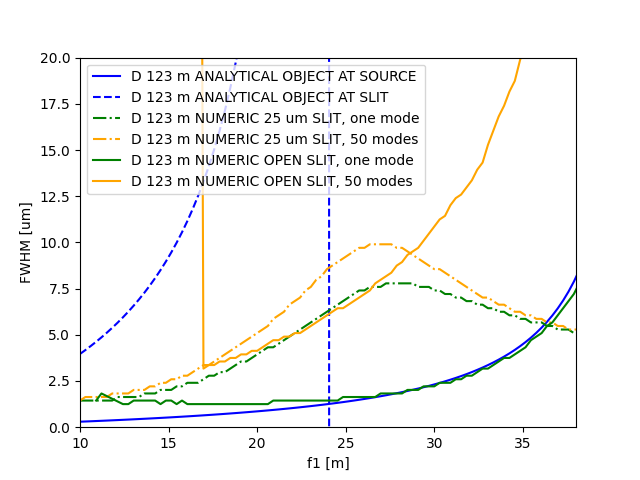
\includegraphics[width=0.95\textwidth]{figures/Figure_magnification_123.png}
    \caption{Magnification obtained by a two transfocator system as a function of focal length of lens 1 $f_1$. The lens 2 focal $f_2$ comes from the trajectories in Fig.~\ref{fig:f1f2map} for $D$~= \SI{99}{\meter}. 
    Analytical values are obtained using equation~\ref{eq:magnification} with $p_1$~= \SI{65}{\meter} (object at source position) (solid lines) or $p_1$~= \SI{30}{\meter} (object at slit position) (dashed lines). Numerical values \ingreen{green} are obtained for the slit (upstream lens 1) either open or closed to $a$~= \SI{25}{\micro\meter}. }
    \label{fig:magnification}
\end{figure}


To simulate a more realistic case, we included partial coherence. Fig.~\ref{fig:sizes} displays the image sizes in the case of coherent source (first coherence mode) and partial coherent source (using 50 coherent modes to mimic the undulator in horizontal).
The most realistic case is the partial coherence case for the \SI{25}{\micro\meter} slit. From the graphics (orange dash-dotted lines) it can be seen that for $D=$~\SI{99}{\meter} (FO1) we obtained a focal spot between 15-35 \SI{}{\micro\meter} \inblue{(11.8-21.6 calculated by Marco)}; and 1.5-10 \SI{}{\micro\meter} \inblue{(15.4-5.3??? calculated by Marco, FO2)} for $D=$~\SI{123}{\meter}.  



\begin{figure}
    \centering
    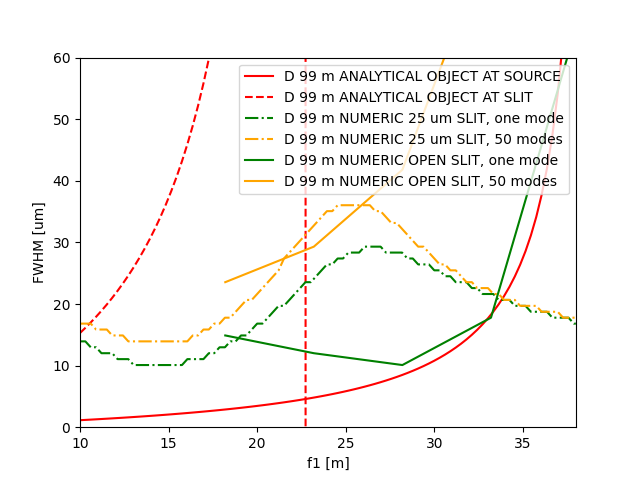
\includegraphics[width=0.95\textwidth]{figures/Figure_sizes_99.png}
    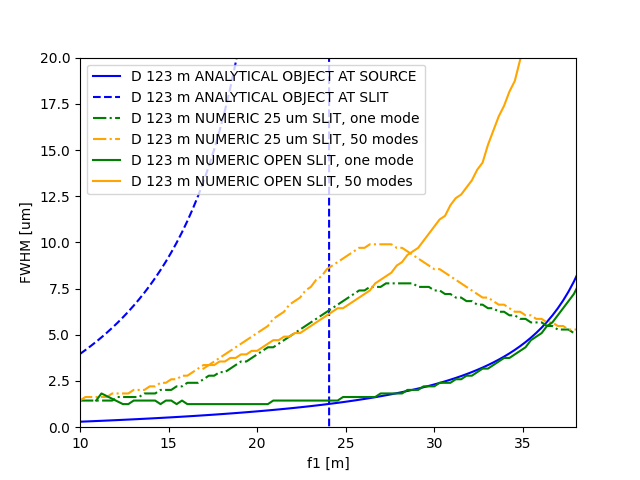
\includegraphics[width=0.95\textwidth]{figures/Figure_sizes_123.png}
    \caption{Beam sizes at the image position (spot at sample) for a two transfocator system as a function of focal length of lens 1 $f_1$. The lens 2 focal $f_2$ comes from the trajectories in Fig.~\ref{fig:f1f2map}.
    Top panel is calculated for \inred{$D$~= \SI{99}{\meter}} and bottom panel with \inblue{$D$~= \SI{123}{\meter}}.
    Numerical values are obtained for the slit (upstream lens 1) either open (solid lines) or closed to $a$~= \SI{25}{\micro\meter} (dash-dotted lines). Simulations are done for a \ingreen{coherent source (green lines)} (\SI{15.14}{\micro\meter} FWHM) and partial coherent source (orange lines) (\SI{71.35}{\micro\meter} FWHM).
    }
    \label{fig:sizes}
\end{figure}


% Some numerical values are in Table~\ref{table:comparison}.
% \begin{table}[]
%     \caption{Simulations}
%     % \label{tab:my_label}
%     \centering
%     \begin{tabular}{ccc}
%          $f_2$ [m] & This work & Marco \\
%         \hline
%          39.7  & 37.00  & 21.5  \\
%          29.38 & 32.19  &   \\
%     \end{tabular}
%     \label{table:comparison}
% \end{table}

     % Appendices appear after the main body of the text. They are prefixed by
     % a single \appendix declaration, and are then structured just like the
     % body text.

\section{Simulations of the complete beamline}

\subsection{1D model (WOFRY)}

\subsection{2D Model (ray-tracing, SRW, COMSYL)}

\section{Discussion}

\section{Summary and conclusions}

\appendix
\section{The Gaussian Shell-model and its use to approximate undulator sources}
\label{sec:appendixA}
The Gaussian Shell-model is a case for partial coherent beams well know in optics, as it models quite well the lasers beams, and it is analytic. It is a 1-dimensional where both the spectral density (intensity distribution) and the degree of transverse coherence between two points follow Gaussian distributions, described by standard deviations $\sigma_I$ and $\sigma_{\mu}$, respectively. The cross spectral density is
\begin{equation}
W(x_1,x_2,\omega) = A^2 e^{-(x_1^2+x_2^2)/(4 \sigma_I^2)} e^{-(x_2-x_1)^2/(2 \sigma_{\mu}^2)}
\label{GS_CSD}
\end{equation}
with $A$, $\sigma_I$ and $\sigma_{\mu}$ positive constants that depend on $\omega$.
This cross spectral density can be decomposed in coherent modes
\cite{Starikov82,mandel_wolf} 
\begin{equation}
W(x_1,x_2,\omega) = \sum_{n=0}^{\infty} \lambda_n(\omega) \Phi^*(x_1,\omega) \Phi(x_2,\omega). 
\label{CMD}
\end{equation}
The $\lambda_n$ (eigenvalues) are
\begin{align}
\lambda_0 &= A \sqrt{\pi/( a+b+c)}; \\ 
\lambda_n &= \lambda_0 q ^n,
\end{align}
with $a = (4 \sigma_I^2)^{-1}$, $ 
b = (2 \sigma_{\mu}^2)^{-1}$, $ 
c = (a^2 + 2 a b)^{1/2}$,
\begin{equation}
q = \frac{1}{1 + \beta^2/2 + \beta\sqrt{(\beta/2)^2+1}} 
\label{q}
\end{equation}
and $\beta=\sigma_{\mu}/\sigma_I$. 

The eigenfunctions are
\begin{equation}
\Phi_n(x) = \left( \frac{2c}{\pi} \right)^{1/4} \frac{1}{\sqrt{2^n n!}} H_n(x\sqrt{2c})e^{-cx^2}
\label{GSeigenvalues}
\end{equation}
with $H_n$ are the physicist's Hermite polynomials of order $n$. 

The occupation of coherent modes, or normalized eigenvalues is   
\begin{equation}
\eta_n = \frac{\lambda_n}{\sum_{i=0}^{\infty} \lambda_i} = q^n(1-q), 
\end{equation}
thus the coherent fraction is $CF=\eta_0=1-q$, and the cumulated occupancy
\begin{equation}
\ \sum_{i=0}^{n-1} \eta_i = 1-q^n. 
\end{equation}
From here one can calculate the number of modes needed to reach a cumulated occupancy $c_0$, which is $n=\ln(1-c_0)/\ln q$.

For representing the undulator radiation by a GSM, we need to obtain the $\sigma_I$ and $\sigma_\mu$ values. The intensity $\sigma_I$ matches the intensity distribution of the undulator source that is usually approximated as the convolution of the electron bunch size $\sigma_x$ with the radiation cross section $\sigma_u$. The other GSM value is $\sigma_\mu=\beta\sigma_I$, and $\beta$ is obtained via $q$ by matching the GSM coherence fraction $CF=1-q$ with the undulator coherence fraction
\begin{equation}
    CF_u = \frac{\sigma_u\sigma_{u'}}{\sqrt{\sigma_x^2+\sigma_u^2}\sqrt{\sigma_{x'}^2+\sigma_{u'}^2}}.
\end{equation}
Therefore, the GSM $\beta$ is obtained by $\beta=CF_u/\sqrt{1-CF_u}$,
and the radiation parameters are $\sigma_{u'}=\sqrt{\lambda/(2L)}$, $L$ the undulator length and $\sigma_u \sigma_{u'} \approx \lambda / (2 \pi)$.




\section{Validity of GSM for coherent mode decomposition of undulator radiation}
\label{sec:appendixB}

We have calculated here the coherent mode decomposition for the U2 undulator (N=100, K=1.19) at the EBS storage ring. 

In a first step the coherent mode decomposition of the undulator radiation has been performed using a 1D model. The results are compared with the GSM approximation. Results for the horizontal direction are in (Fig.~\ref{fig:GSMvsUND-H}) in (Fig.~\ref{fig:GSMvsUND-V}) for the vertical one. As expected, these figures shows that the GASm is a good approximation for cases where the coherence fraction is small (the horizontal case) but the results are very different, in particular the eigenfunctions, in the case of high coherence (vertical direction in Fig.~\ref{fig:GSMvsUND-V}).


\begin{figure}
    \centering
    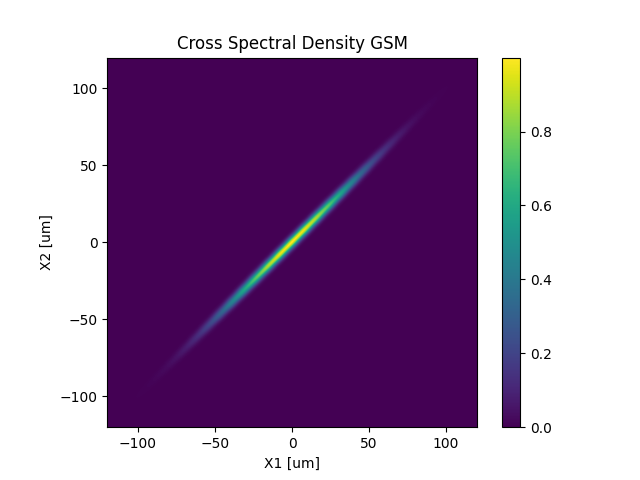
\includegraphics[width=0.49\textwidth]{figures/comparison_H_CSD_GSM.png}
    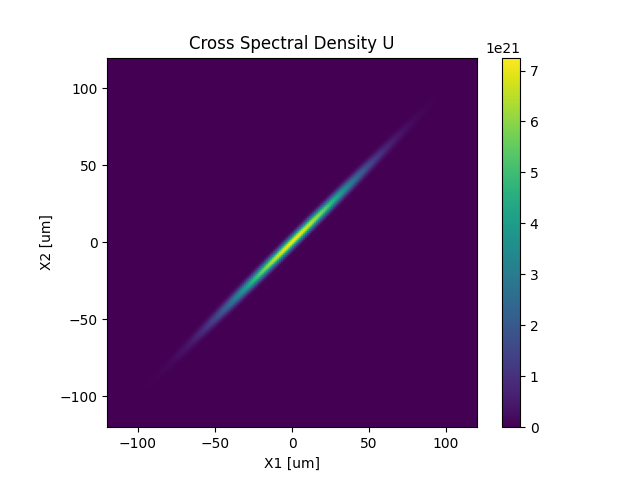
\includegraphics[width=0.49\textwidth]{figures/comparison_H_CSD_U.png}
    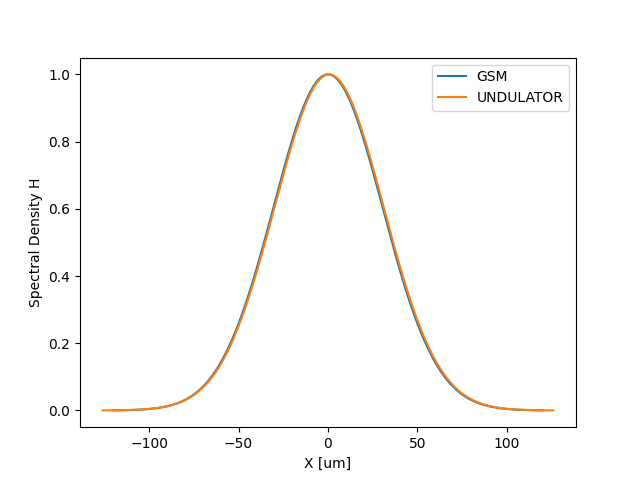
\includegraphics[width=0.59\textwidth]{figures/comparison_H_SD.png}
    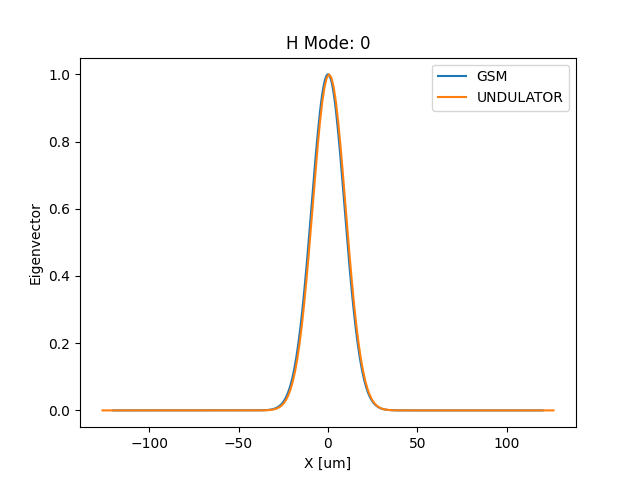
\includegraphics[width=0.49\textwidth]{figures/comparison_H_eigenvector0.png}
    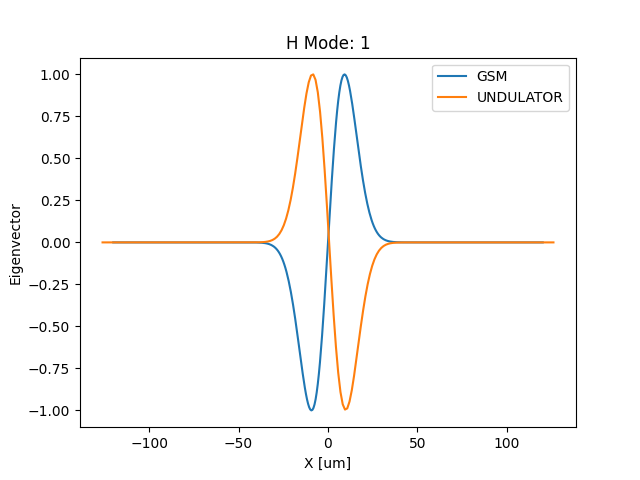
\includegraphics[width=0.49\textwidth]{figures/comparison_H_eigenvector1.png}
    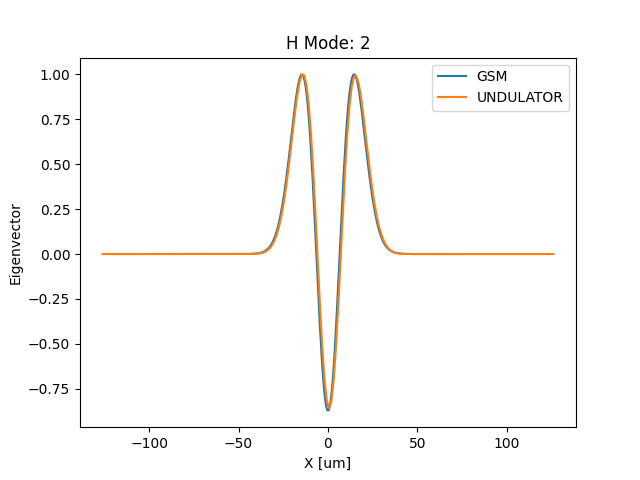
\includegraphics[width=0.49\textwidth]{figures/comparison_H_eigenvector2.png}
    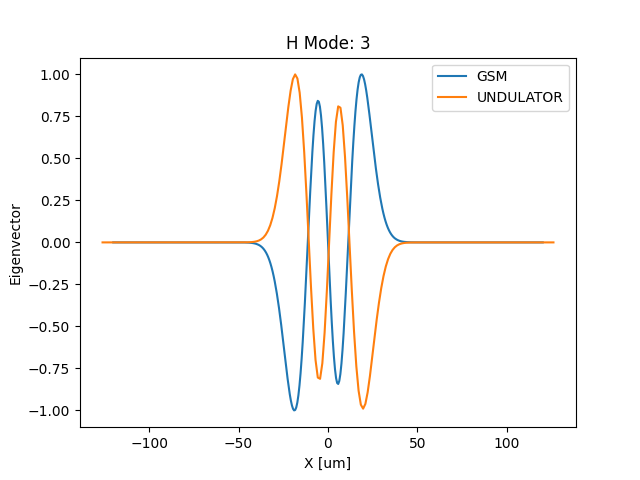
\includegraphics[width=0.49\textwidth]{figures/comparison_H_eigenvector3.png}
        
    \caption{Comparison of the approximated (GSM) and exact (1D WOFRY) coherent mode decomposition  for the Horizontal direction of a U20 undulator of length \SI{2}{\meter},  set to resonance at 10 keV photon. energy. The plot show the Cross Spectral Deisity, Spectral Density, and four first modes. The Coherence Fraction is 0.088}
    \label{fig:GSMvsUND-H}
\end{figure}


\begin{figure}
    \centering
    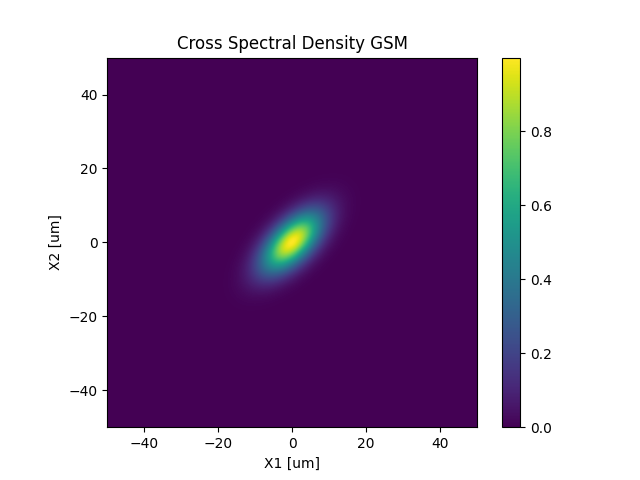
\includegraphics[width=0.49\textwidth]{figures/comparison_V_CSD_GSM.png}
    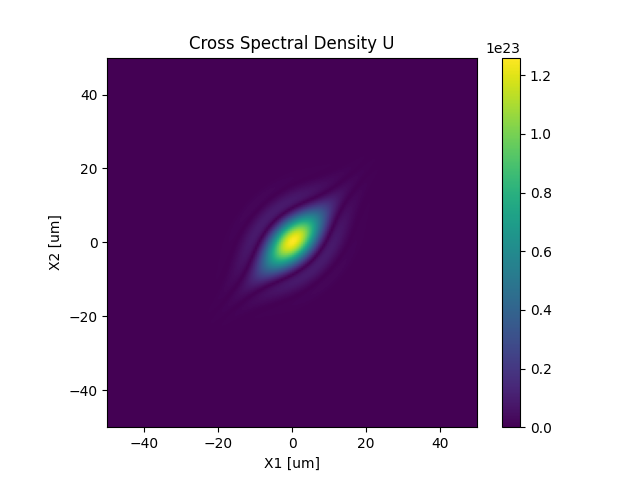
\includegraphics[width=0.49\textwidth]{figures/comparison_V_CSD_U.png}
    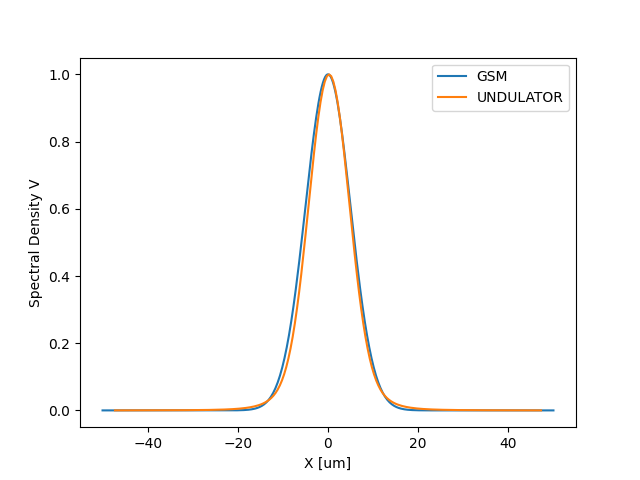
\includegraphics[width=0.59\textwidth]{figures/comparison_V_SD.png}
    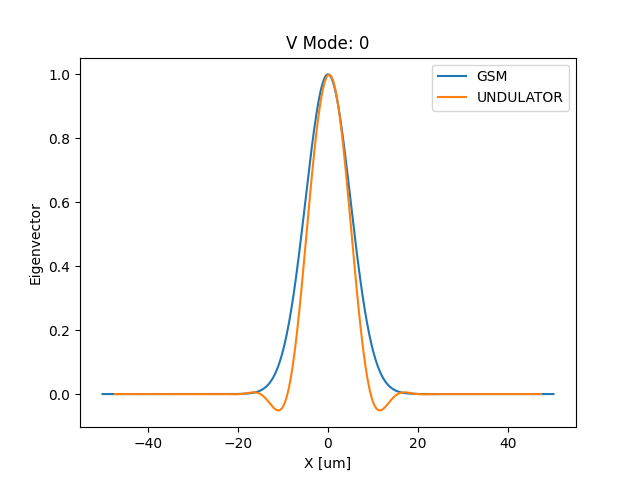
\includegraphics[width=0.49\textwidth]{figures/comparison_V_eigenvector0.png}
    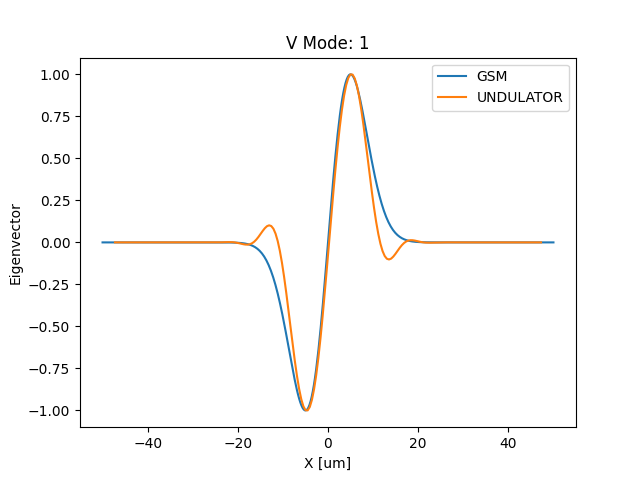
\includegraphics[width=0.49\textwidth]{figures/comparison_V_eigenvector1.png}
    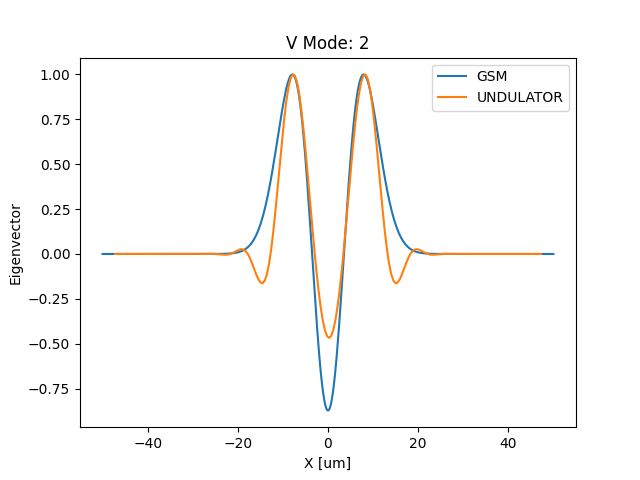
\includegraphics[width=0.49\textwidth]{figures/comparison_V_eigenvector2.png}
    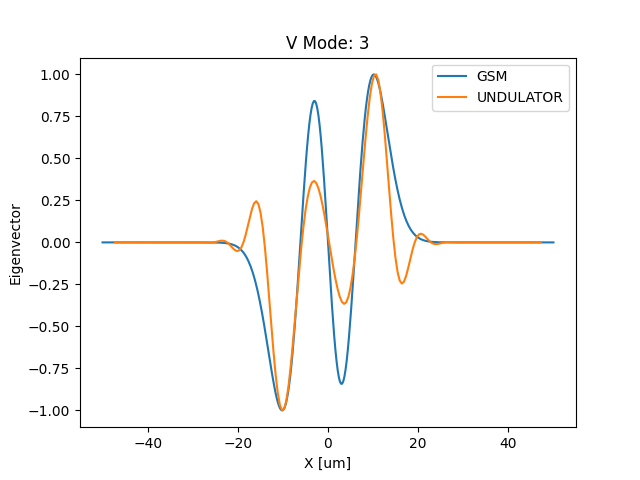
\includegraphics[width=0.49\textwidth]{figures/comparison_V_eigenvector3.png}
        
    \caption{The same as Fig.~\ref{fig:GSMvsUND-H} but for the vertical direction. The Coherence Fraction is 0.665}
    \label{fig:GSMvsUND-V}
\end{figure}



Next step is the analysis of the separability in horizontal and vertical. In Fig.~\ref{fig:GSMvsCOMSYL} we compare the coherent fraction calculated with COMSYL \cite{comsyl} and approximated by GSM (as shown in Appendix~\ref{sec:appendixA}). It shows that the GSM approximated well an undulator only for the fist modes. The Coherent Fraction (first mode) matches very well. This is due to the fact that the GSM approximation to the undulator is built matching the CF. The occupancy of higher modes differ: the first 50 GSM modes GSM to contain more than 99\% of the spectral density, but XX are needed for the numerical coherent mode decomposition with COMSYL. This means significative errors in the eigenvalues when using GSM. 

\todo{Compare COMSYL with H+V combination of WOFRY1D modes}


\begin{figure}
    \centering
    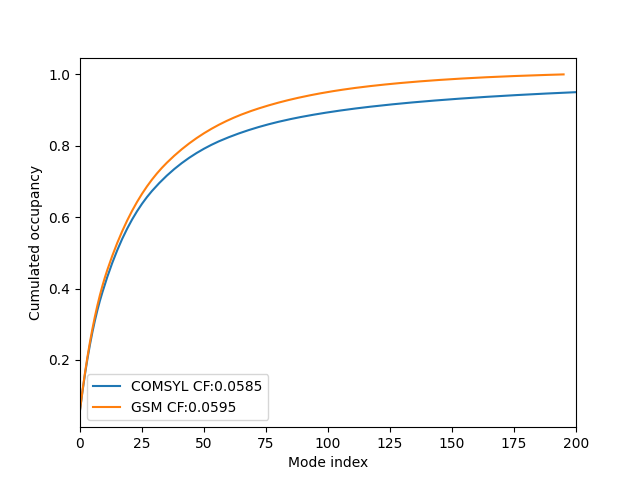
\includegraphics[width=0.95\textwidth]{figures/FigureGSMvsCOMSYL.png}
    \caption{Comparison of the approximated (GSM) and exact (COMSYL) cumulated occupation of the coherent modes for an undulator U20, of length \SI{2}{\meter}, and set to resonance at 10 keV photon. energy.}
    \label{fig:GSMvsCOMSYL}
\end{figure}

\section{Testing the effect of a slit in the GSM}
\label{appendix:B}

In many cases the use of the GSM supposes that during propagation over the beamline elements the beam keeps its Gaussian Shell-model nature. This is true for propagation in free space, and probably true for focusing with ideal lenses. But, in the case of slits that crop the beam, it is difficult to believe that the beam is still Gaussian. Moreover, the new beam parameters $\sigma_{I'}$ and $\sigma_{\xi'}$ are obtained supposing the slit has a width $\sigma_s$, applying
\begin{equation}
    \frac{1}{\sigma_{I'}^2} = 
    \frac{1}{\sigma_{I}^2} +
    \frac{1}{\sigma_{s}^2},
\end{equation}
and
\begin{equation}
    \sigma_{\xi'} = \sigma_{\xi} 
\end{equation}

However, there are several recipes for the relation between $\sigma_s$ and the slit aperture $A$: $\sigma_s=A/4.1$, $\sigma_s=A/2.355$ and $\sigma_s=A/\sqrt{12}$.

We have calculated the case of a Gaussian beam that is cropped by a slit. The exact calculation is compared with the GSM results using the different recipes. We have used $\sigma_x$~= \SI{30}{\micro\meter} (like for the H EBS source) and three possible values of $\beta$: quite incoherent ($\beta=0.02$), medium coherence ($\beta=0.09$) and quite coherent ($\beta=1.15$). The results are in Fig.~\ref{fig:GSMslit} where the CF is compared for the exact calculation and the GSM approximation. We remind that the CF for the GSM is $CF = 1 - q$, with $q$ given in equation~\ref{q}.
The source has been created using the GSM model with a sufficient number of modes to include more that 99\% of the spectral density. Each mode is cropped by the slit placed at the source position. The Cross Spectral Density $W$ is calculated in the usual way 
\begin{equation}
    W(x_1,x_2) = \sum \lambda_i \Phi^*(x_1) \Phi(x_2),     
\end{equation}
with $\lambda_i$ the eigenvalues of the source and $\Phi(x_{1,2})$ are the eigenvectors of the source cropped by the slit. After re-diagonalizing $W$, the new eigenvalues $\lambda_i'$ permit to calculate the exact CF: 
\begin{equation}
    CF = \frac{\lambda_0'}{\sum \lambda_i'}
\end{equation}

The results in Fig.~\ref{fig:GSMslit} show two important things:
i) the GSM model usually overestimates CF in particular for high coherence ($\beta=1.15$), where there are important discrepancies between GSM and the exact calculation.
ii) For low coherence the GSM may work, in particular when using the aperture $\sigma_s=A/2.355$, i.e., matching the Gaussian FWHM with the total aperture.

\begin{figure}
    \centering
    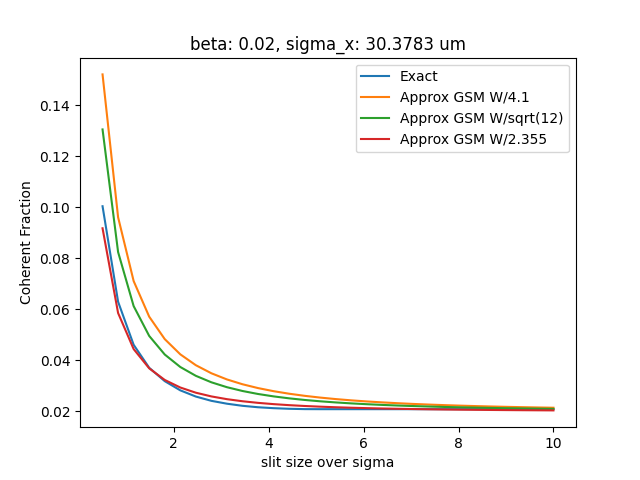
\includegraphics[width=0.95\textwidth]{figures/Figure_1a.png}
    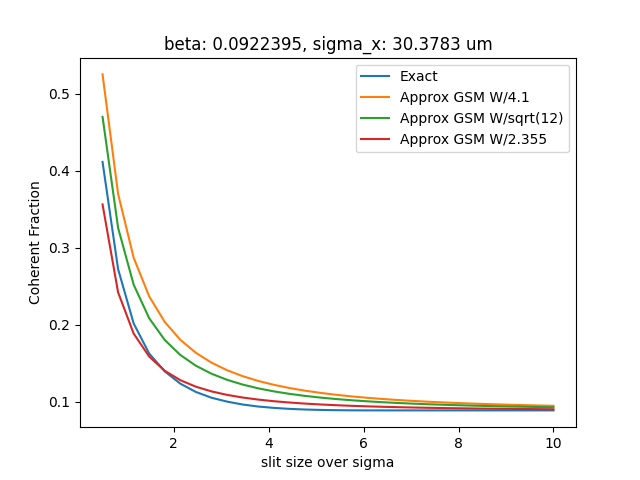
\includegraphics[width=0.95\textwidth]{figures/Figure_1b.png}
    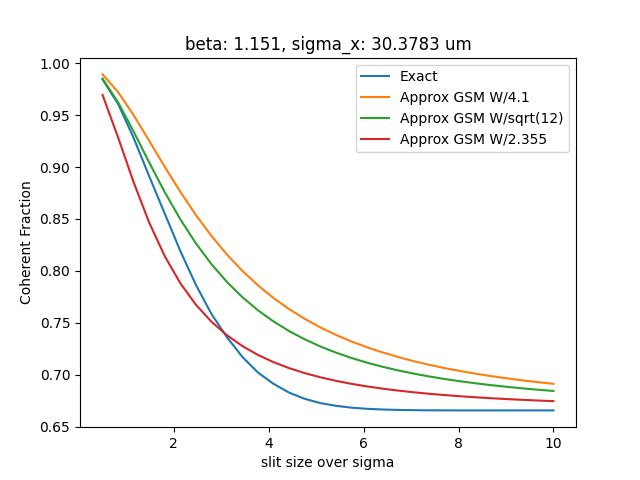
\includegraphics[width=0.95\textwidth]{figures/Figure_1c.png}
    \caption{Calculation of the coherence fraction f a Gaussian beam cropped by a slit. The exact numerical laculation (blue line) is compared with the approzimations that the beam is still described by a GSM with three possible ways to calculate the slit ``Gaussianized" $\sigma_s$ (see text). }
    \label{fig:GSMslit}
\end{figure}


\section{One lens: comparison of methods}


\begin{figure}
    \centering
    \includegraphics[width=0.95\textwidth]{figures/oneTFund_400um.eps}
    % \includegraphics[width=0.95\textwidth]{figures/oneTFund_300um.png}  
    \includegraphics[width=0.95\textwidth]{figures/oneTFund_200um.eps}
    % \includegraphics[width=0.95\textwidth]{figures/oneTFund_100um.png}

    \caption{Evolution of the size of a coherent undulator beam cropped by a slit and focused by a lens of different radii valyes $R$: a) \SI{400}{\micro\meter} and b) \SI{200}{\micro\meter}.
    
    }
    \label{fig:oneTFundAppendixR}
\end{figure}



\begin{figure}
    \centering
    
    a) Und + RectSlit + RealLens \\
    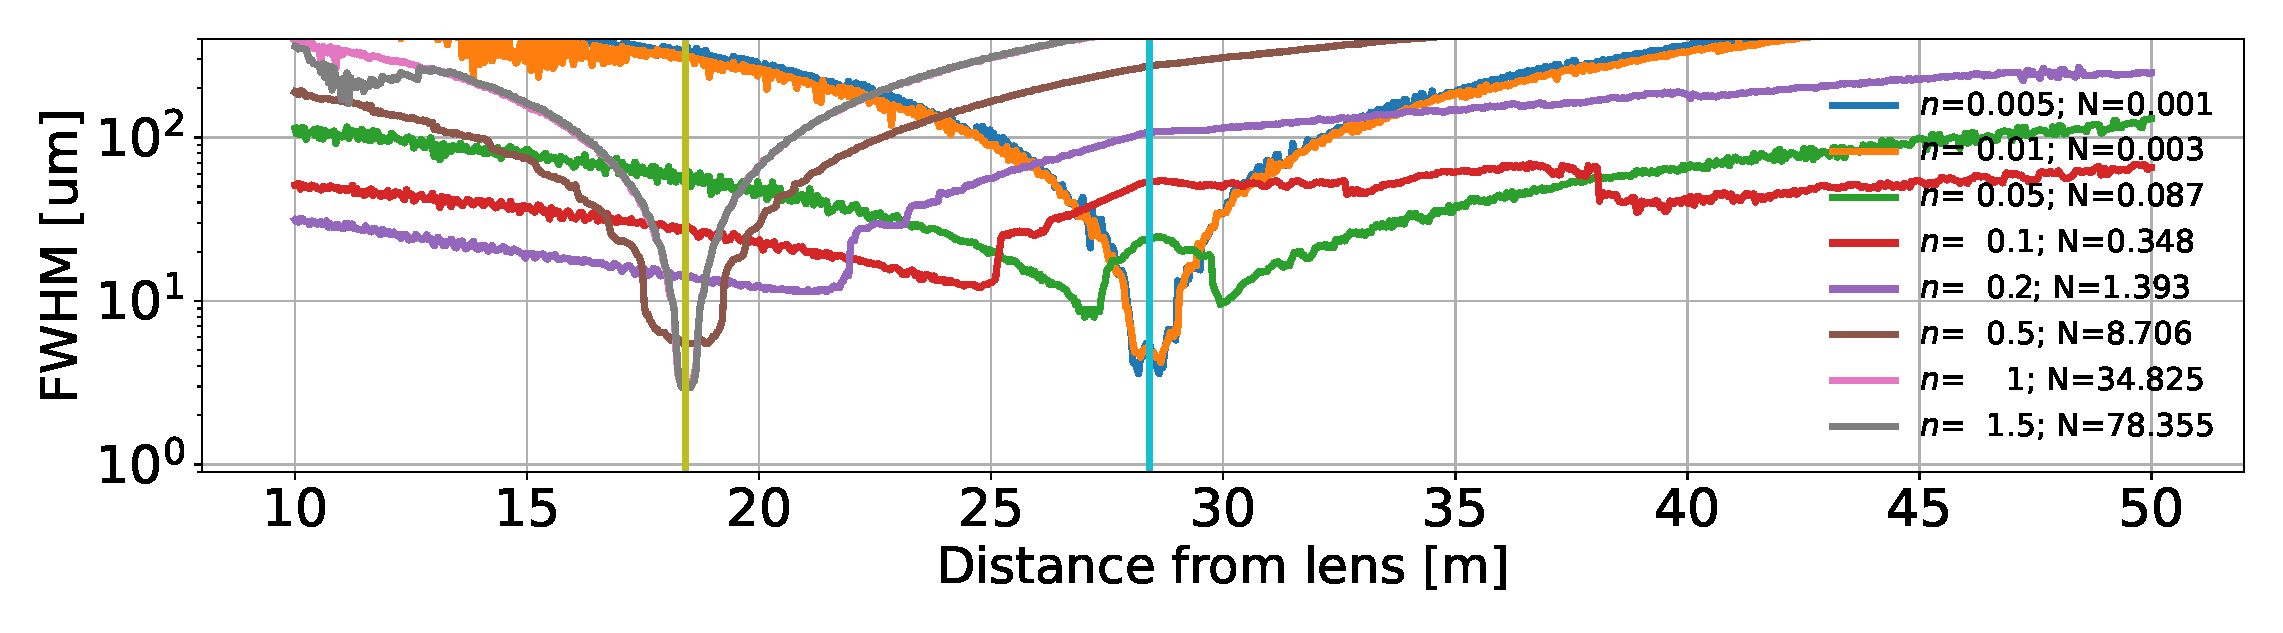
\includegraphics[width=0.95\textwidth]{figures/oneTF_UndSource_RectSlit_R200um.eps}
    
    b) Gauss + RectSlit + RealLens \\
    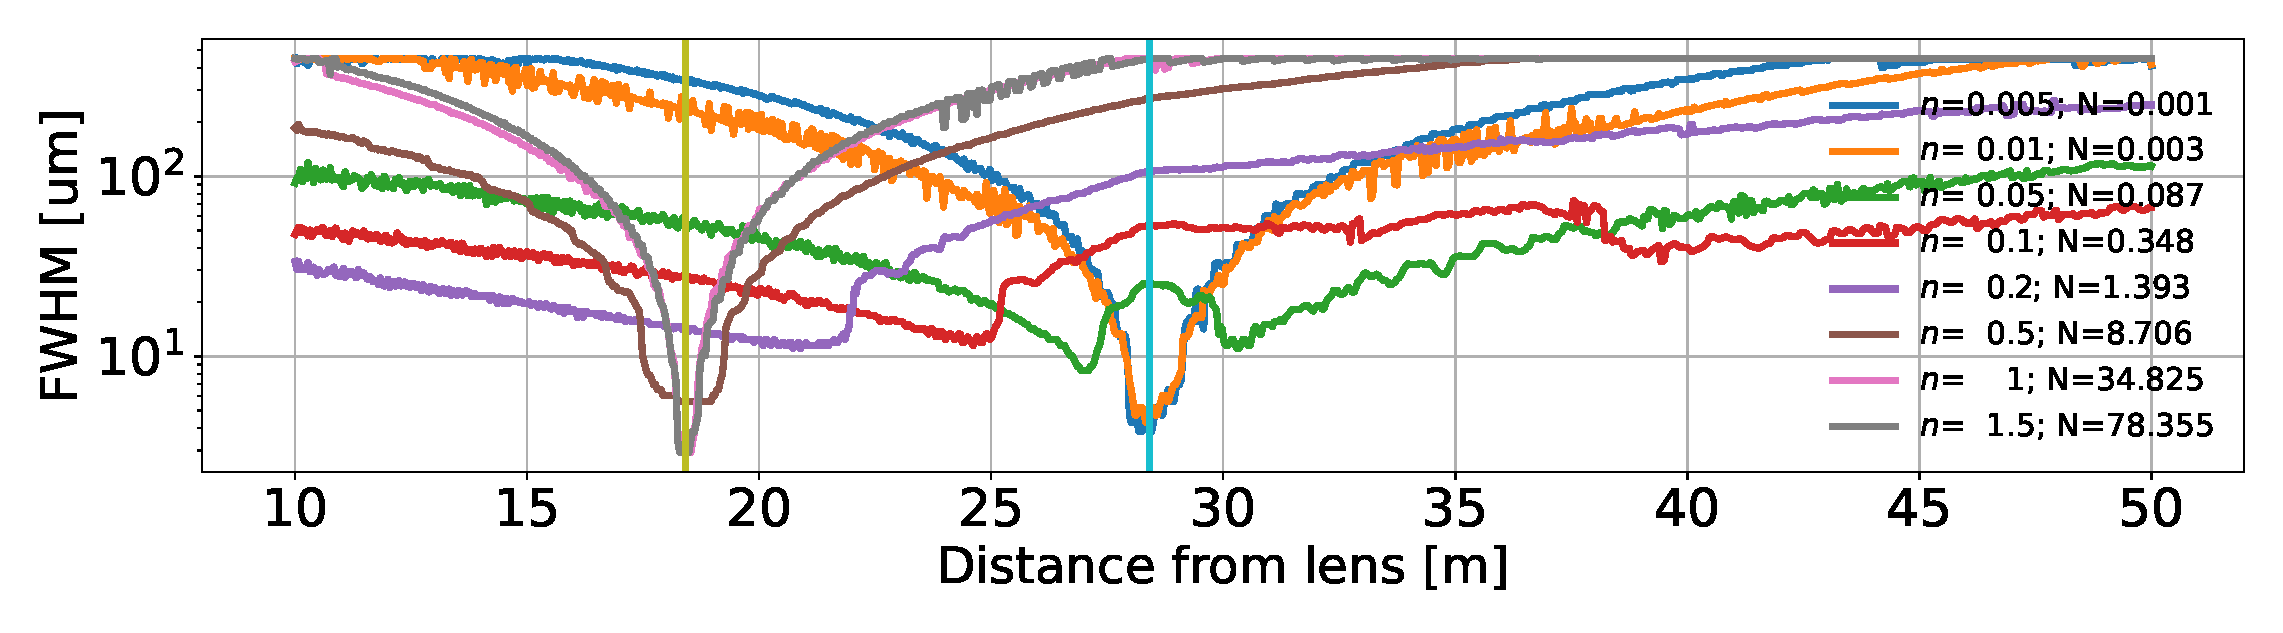
\includegraphics[width=0.95\textwidth]{figures/oneTF_GaussianSource_RectSlit_R200um.eps}
    
    c) Gauss + GaussSlit + RealLens \\
    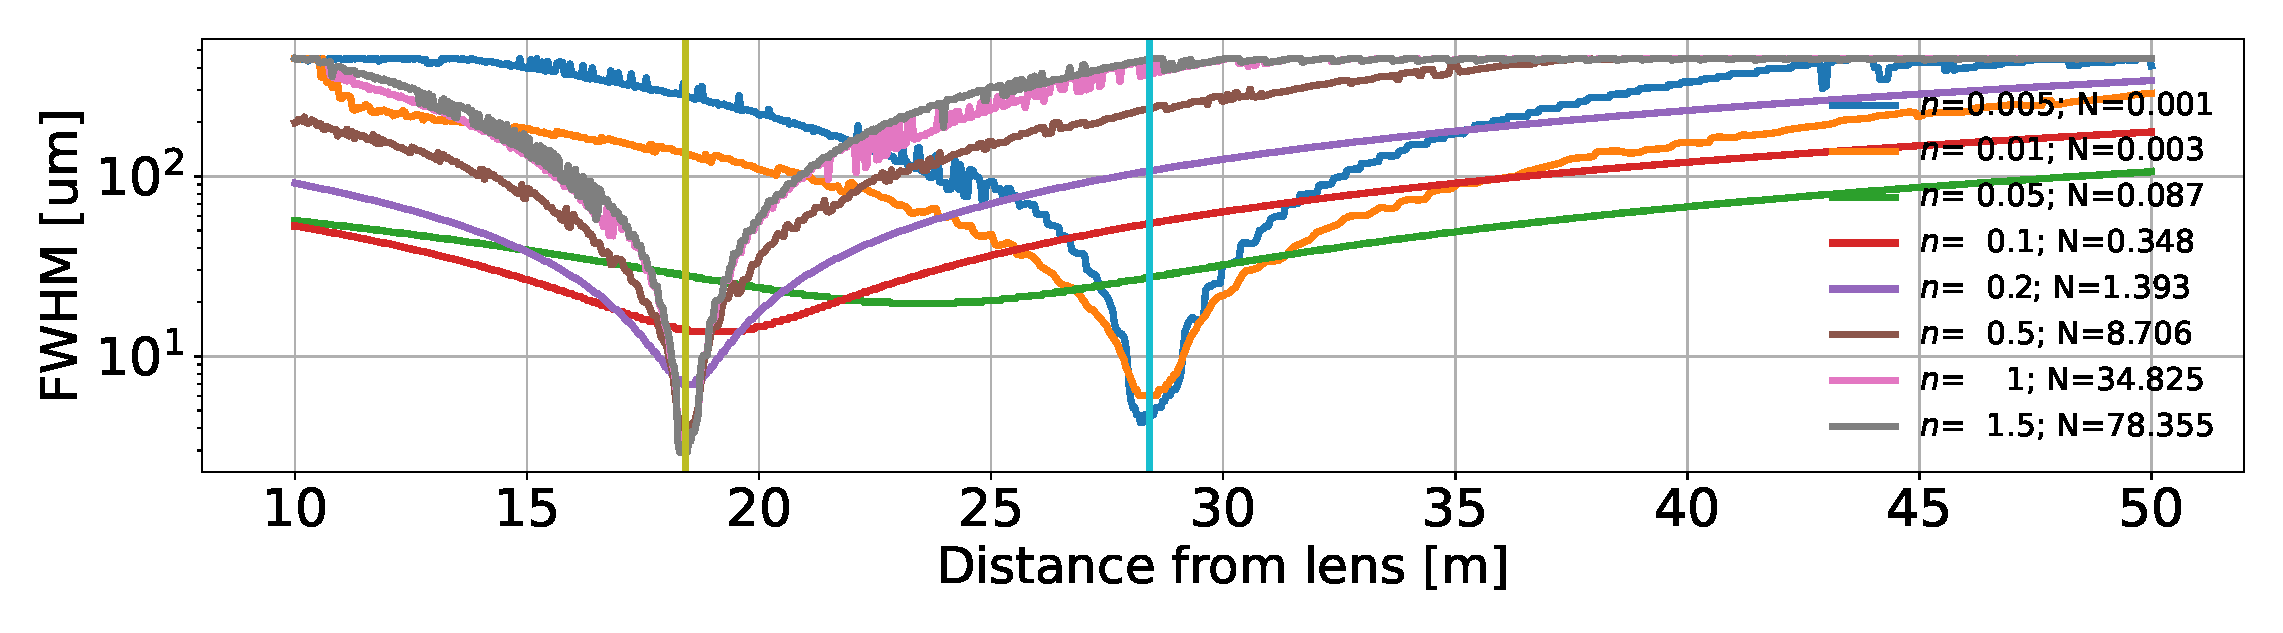
\includegraphics[width=0.95\textwidth]{figures/oneTF_GaussianSource_GaussianSlit_200um.eps}

    d) Gauss + GaussSlit + IdealLens \\
    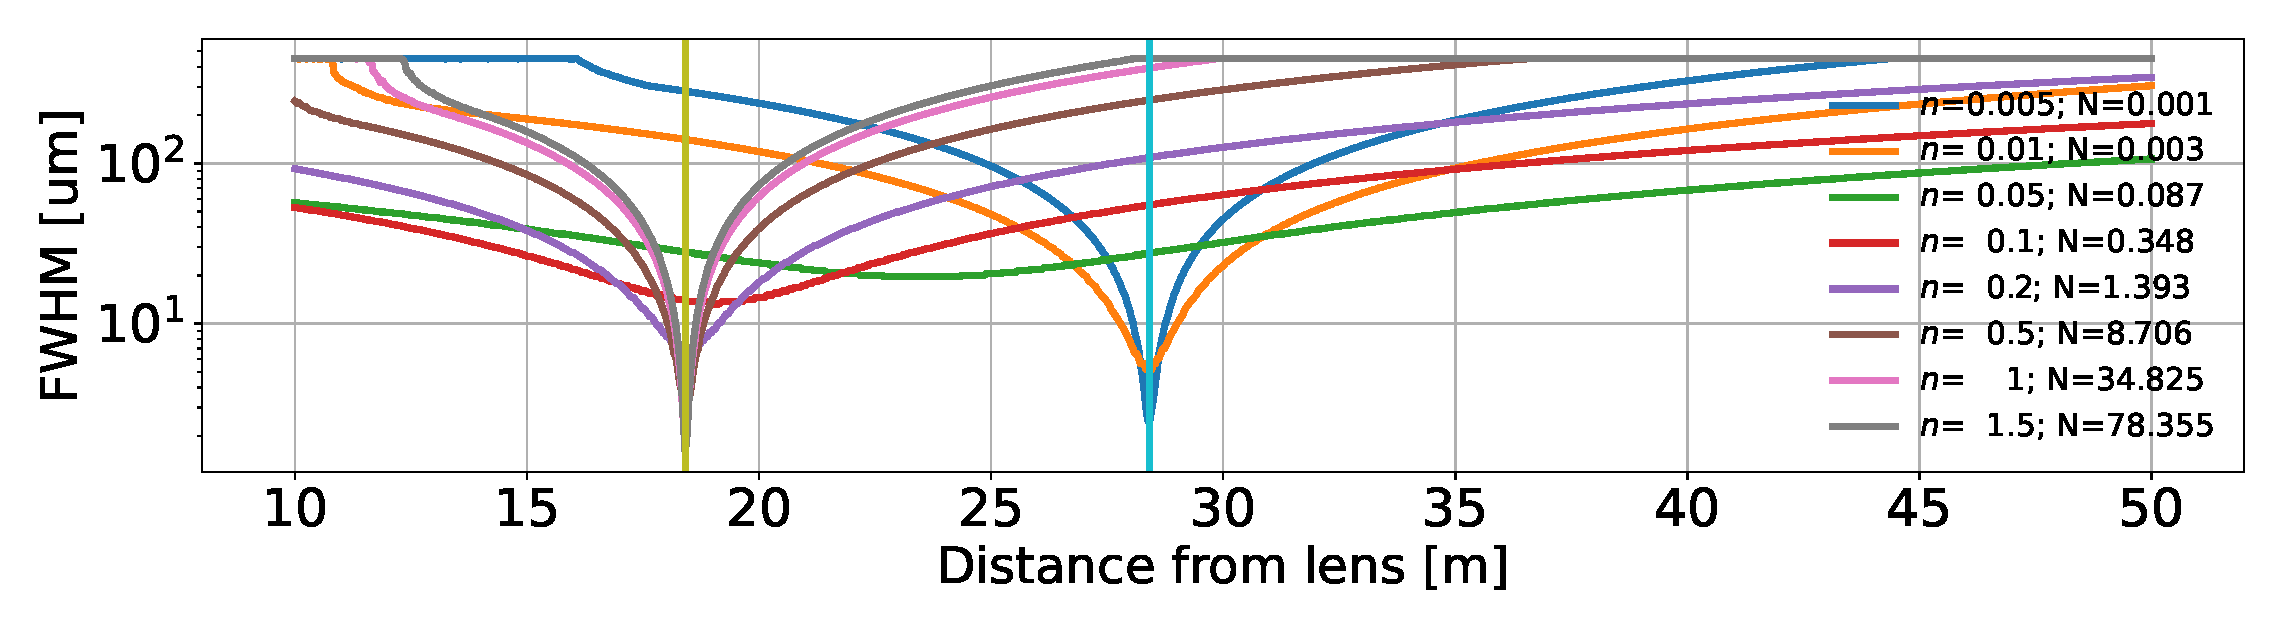
\includegraphics[width=0.95\textwidth]{figures/oneTF_GaussianSource_GaussianSlit_IdealLens.eps}
    
    e) Hybrid (Und + RectSlit + RealLens) \\
    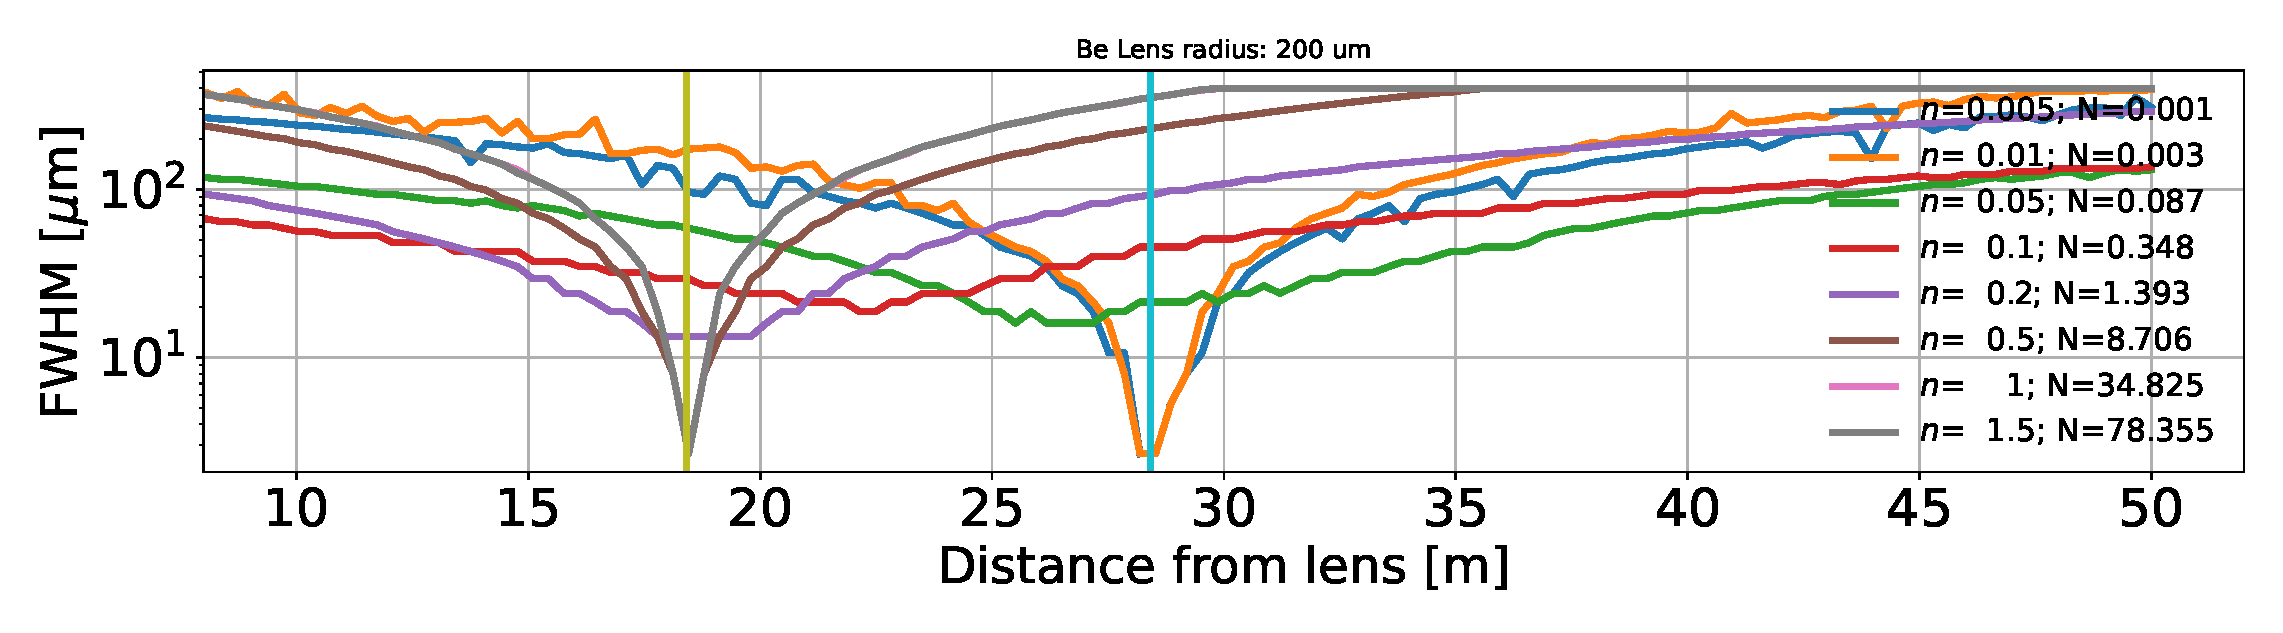
\includegraphics[width=0.95\textwidth]{figures/oneTF_ShadowHybrid_R200um.eps}
    
    \caption{Evolution of the size of a coherent undulator beam cropped by a slit and focused by a lens of $R$=~\SI{0.2}{\milli\meter} using different methods: 
    
    a) Undulator source + Rectangular Slit + Real Lenses
    
    b) Gaussian source + Rectangular Slit + Real Lenses
    
    c) Gaussian source + Gaussian Slit + Real Lenses
        
    d) Gaussian source + Gaussian Slit + Ideal lens (Full Gaussian)
        
    e) Ray tracing, hybrid, with undulator source + Rectangular Slit + Real Lenses.
    }
    \label{fig:oneTF_comparison}
\end{figure}


\begin{figure}

    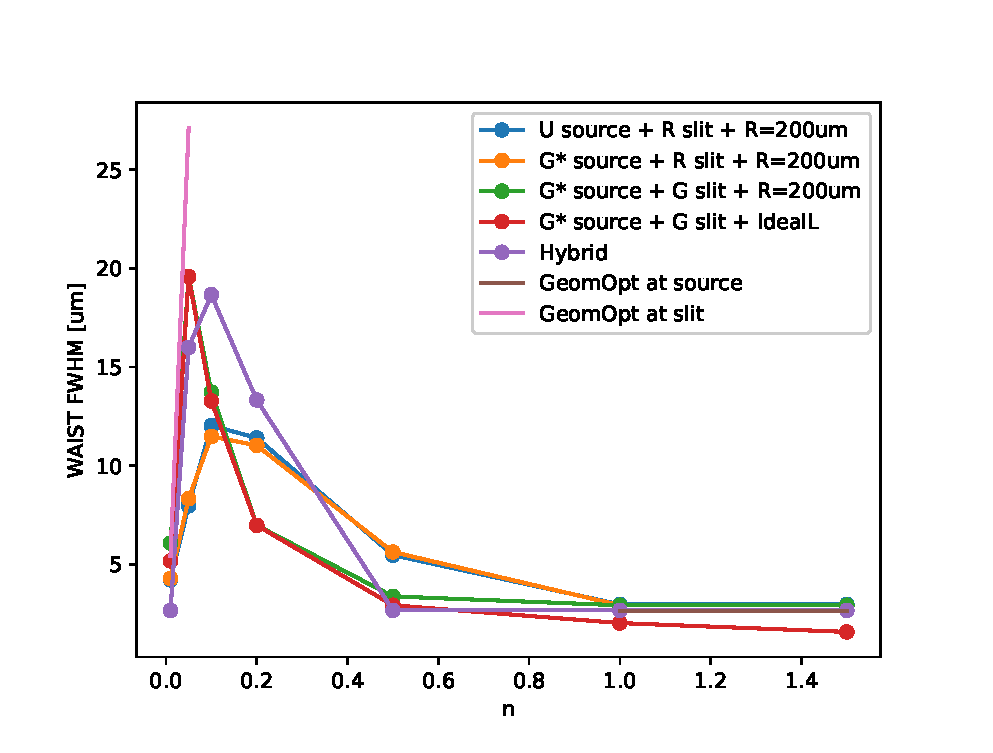
\includegraphics[width=0.95\textwidth]{figures/waist_size_comparison.eps}
    
    \caption{Waist size vs slit aperture for the different methods studied. 
    
    }
    \label{fig:oneTFund}
\end{figure}



\section{OLD PART FOR ONE LENS}

We have calculated the beam evolution using wave optics. The source has $\sigma_s=$\SI{15.3/2.355}{\micro\meter} and $\lambda=$\SI{1.2}{\AA}, and the lens $p=$\SI{65}{\meter}, $f=$\SI{28.2}{\meter}, and a slit of variable aperture $a$ is placed at $p_a$=\SI{30}{\meter} from the lens. The beam at the slit plane has a size $\sigma_a=$\SI{125}{\micro\meter} \todo{CHECK WITH FORMULAS...} and the aperture is open at $a = n \sigma_a$ with $n=6,4,2,1.5,1,0.5,0.2,0.1$. The cross section of the beam is defined by i) the full-width at half-maximum (FWHM) of the intensity distribution, or also ii) the on-axis intensity $I_{axis}$. At the focal position, the FWHM should present a minimum and $I_{axis}$ a maximum. 

The slit is implemented in two ways. First, as a Gaussian appodization window for the beam intensity. This guarantees the validity of regime (2) in the previous section. The FWHM of the weighting  Gaussian window corresponds to the slit aperture $a$. This is the value that better approximates a slit by a Gaussian window, as discussed in Appendix~\ref{sec:appendixC}. Second, in a  more realistic model, the slit is acting as a transmission window of rectangular shape with width $a$. 

Fig.~\ref{fig:oneTFG}a shows the evolution of the beam after being focused by the lens. With the open slit the geometrical optics give a focal position $q=$\SI{49.81}{\meter} (source at $p$) and $q'=$\SI{470}{\meter} (source at $p_a$ slit). \todo{CALCULATE AND COMPARE FOCAL SIZES} 


\begin{figure}
    \centering
    %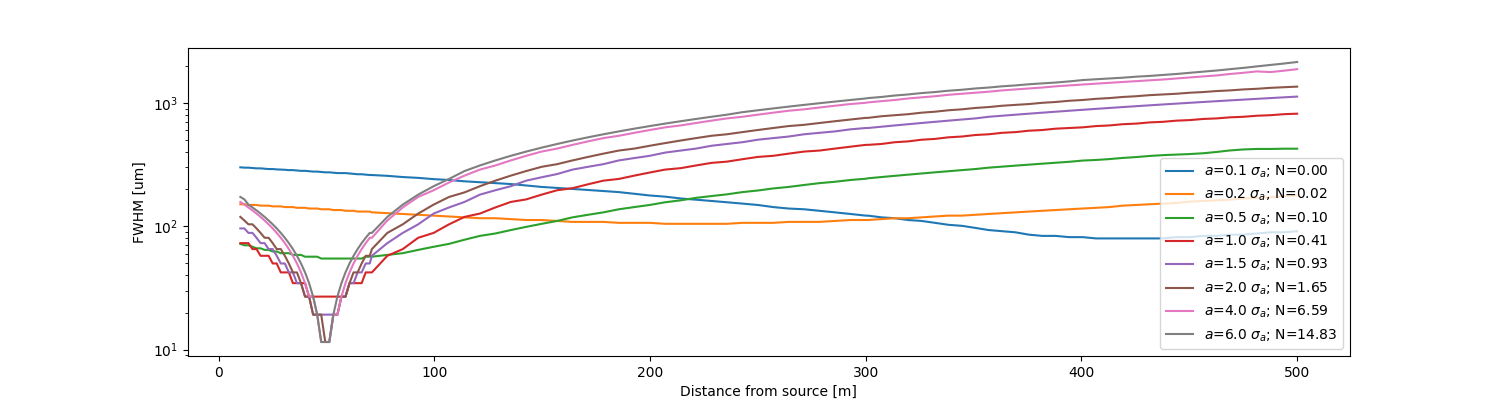
\includegraphics[width=0.95\textwidth]{figures/FigureG_1.png}
    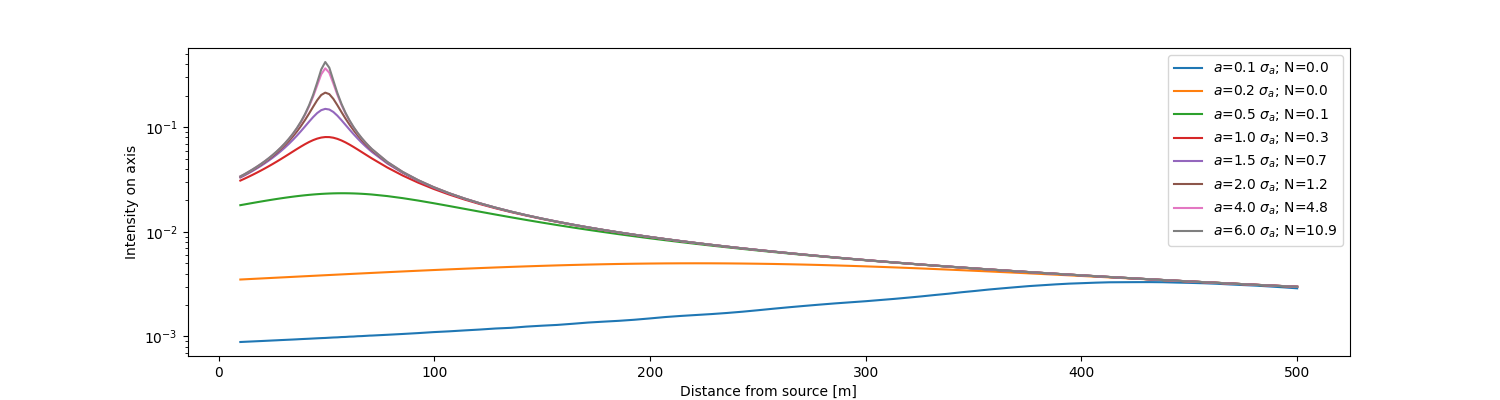
\includegraphics[width=0.95\textwidth,height=5cm]{figures/FigureG_2.png}
    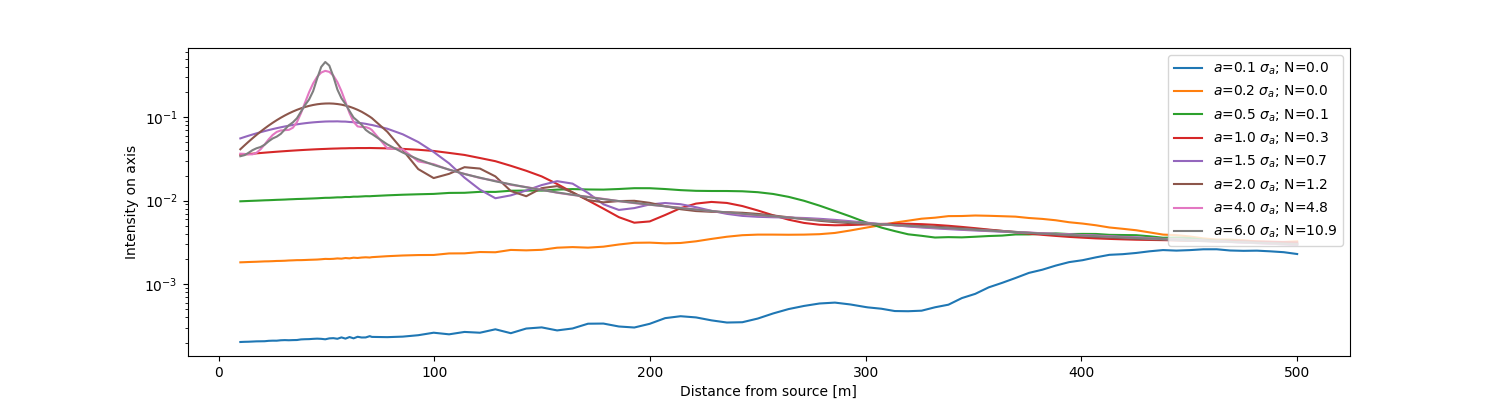
\includegraphics[width=0.95\textwidth,,height=5cm]{figures/Figure_2.png}
    \caption{Evolution of a beam cropped by a slit and refracted by a lens as a function of the distance from the lens.
    %a) evolution of the FWHM of the beam size, 
    The plot shows the evolution of the intensity on-axis. The aperture is open at $a = n \sigma_a$ with $n=6,4,2,1.5,1,0.5,0.2,0.1$, $\sigma_a=$\SI{125}{\micro\meter}. The waist is found at a maximum of the intensity on-axis. The Fresnel number of the slit is also marked in the legend.
    a) the slit is modelled as a Gaussian window,
    b) the slit is modelled by a rectangular function.}
    \label{fig:oneTFG}
\end{figure}

 
However, in real life the slit cannot be approximated by a Gaussian appodization window, but a rectangular-shaped function. This has important consequences: when the slit crops significantly the beam the Gaussian beam regime is broken therefore numerical calculation are necessary. Fig.~\ref{fig:oneTFG}b shows the beam evolution in this case.  It can be noticed that for $n=$6 or 4 ($N=$14, 6, respectively) the situation does not change with respect to Fig.~\ref{fig:oneTFG}a because the slit very slightly crops the beam. For $n=2.0$ ($N=1.65$) the peak intensity at the waist reduces (although not changing position) and the evolution versus distance becomes wavy because the slit diffraction create new peaks in the beam intensity profile. 

\inblue{These calculations show how important is to model the apertures using a realistic (rectangular) function. The Gaussian approximation of the apertures does not reproduce the expected beam evolution. }

The next step is to consider a partial coherent source. For that, we used a Gaussian Shell-model (GSM) with parameters obtaining by matching the coherence fraction of the undulator source (see Appendix~\ref{sec:appendixA}). Indeed, the source used until here was the first coherence mode of such a source, that represents an approximation of the undulator in horizontal plane. Repeating the calculations shown for partial coherence (adding a number of modes that represent the full beam) we obtained no changes in the position of the best focus. There are however important changes in the waist dimensions and small changes in intensity. These are illustrated in Fig.~\ref{fig:waist}. \todo{comment the reduction of the intensity}

\begin{figure}
    \flushleft
% ~~~~a)~~~~~~~~~~~~~~~~~~~~~~~~~~~~~~~~~~~~~~~~~~~~~~b)\\
    \centering
    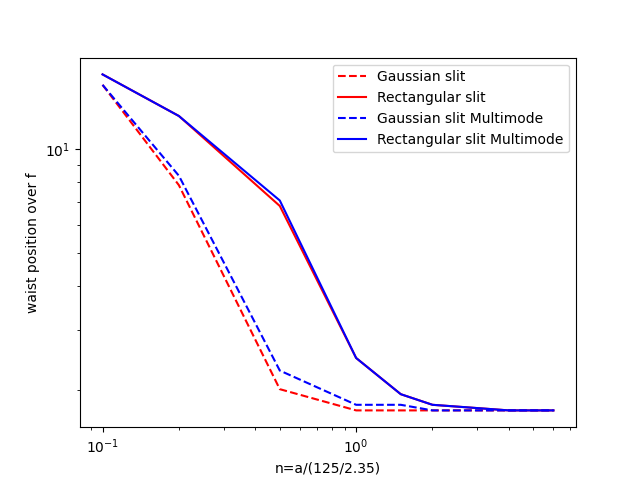
\includegraphics[width=0.75\textwidth]{figures/FigureW1.png}
    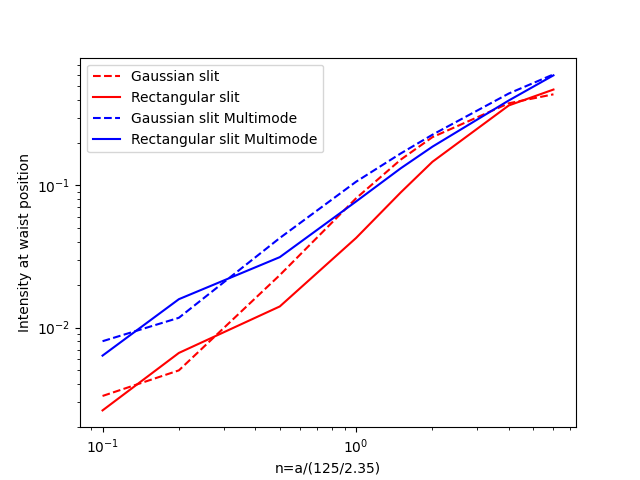
\includegraphics[width=0.75\textwidth]{figures/FigureW2.png}
    \flushleft
% ~~~~c)~~~~~~~~~~~~~~~~~~~~~~~~~~~~~~~~~~~~~~~~~~~~~~d)\\
    \centering
    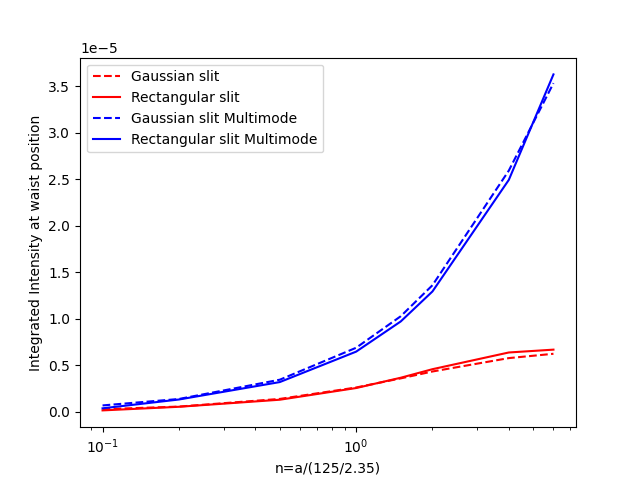
\includegraphics[width=0.75\textwidth]{figures/FigureW3.png}
    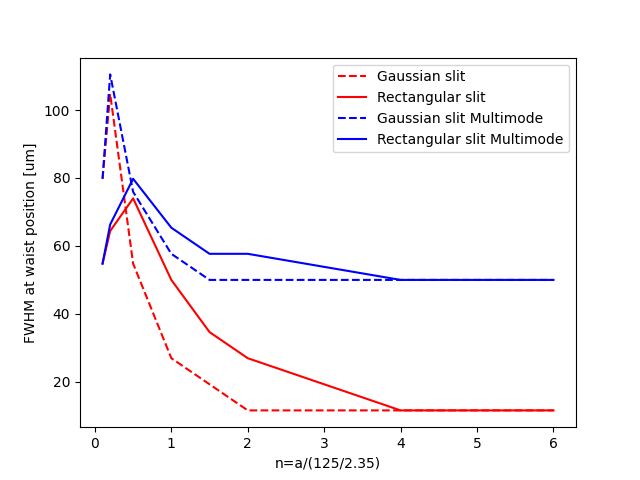
\includegraphics[width=0.75\textwidth]{figures/FigureW4.png}
    \caption{Parameters of the beam waist (position, size, intensity) versus slit aperture (measured in $\sigma_a$ units for the first Gaussian mode).  a) waist position, b) on axis intensity, c) integrated intensity and d) waist size in FWHM.}
    \label{fig:waist}
\end{figure}


\todo{Discuss the effect of real lens: No main differences because the focusing effect needed can be obtained using only a single Be lens}

We want also to calculate the cross section dimension of the beam at a given plane, even if this plane is not at the focal position, and how it changes with the slit opening. This would would be useful to match the acceptance if a second transfocator is to be placed in that plane. Fig. \ref{fig:slit99m} shows the cross section of the beam at a plane placed at $d$~= \SI{99}{\meter} downstream from the lens. It shows that the cross section reduces as the slit aperure closes, and passes trough a minimum when the ``moving" focal position goes trough this plane. However, this happens for a different aperture size when comparing the Gaussian slit and the Rectangular slit. The positions for the coherent beam or the partial coherent beam coincide in position, but not exactly in size.


\begin{figure}
    \centering
    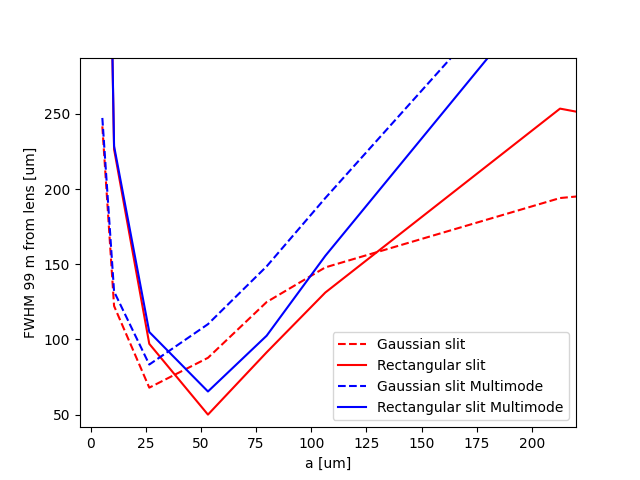
\includegraphics[width=0.95\textwidth]{figures/Figure99m.png}
    \caption{Beam size at a plane placed at \SI{99}{\meter} downstream from the lens as a function of the slit opening.}
    \label{fig:slit99m}
\end{figure}




     %-------------------------------------------------------------------------
     % The back matter of the paper - acknowledgements and references
     %-------------------------------------------------------------------------

     % Acknowledgements come after the appendices

\ack{Acknowledgements}

     % References are at the end of the document, between \begin{references}
     % and \end{references} tags. Each reference is in a \reference entry.

% \begin{references}
% \reference{Author, A. \& Author, B. (1984). \emph{Journal} \textbf{Vol}, 
% first page--last page.}
% \end{references}
% \cite{knuth84}

%% Note added by Overleaf: If using bibtex, remove the "references" environment above, and uncomment the following lines.
\bibliographystyle{iucr}
\referencelist{iucr}

     %-------------------------------------------------------------------------
     % TABLES AND FIGURES SHOULD BE INSERTED AFTER THE MAIN BODY OF THE TEXT
     %-------------------------------------------------------------------------

     % Simple tables should use the tabular environment according to this
     % model

% \begin{table}
% \caption{Caption to table}
% \begin{tabular}{llcr}      % Alignment for each cell: l=left, c=center, r=right
%  HEADING    & FOR        & EACH       & COLUMN     \\
% \hline
%  entry      & entry      & entry      & entry      \\
%  entry      & entry      & entry      & entry      \\
%  entry      & entry      & entry      & entry      \\
% \end{tabular}
% \end{table}

     % Postscript figures can be included with multiple figure blocks

% \begin{figure}
% \caption{Caption describing figure.}
% 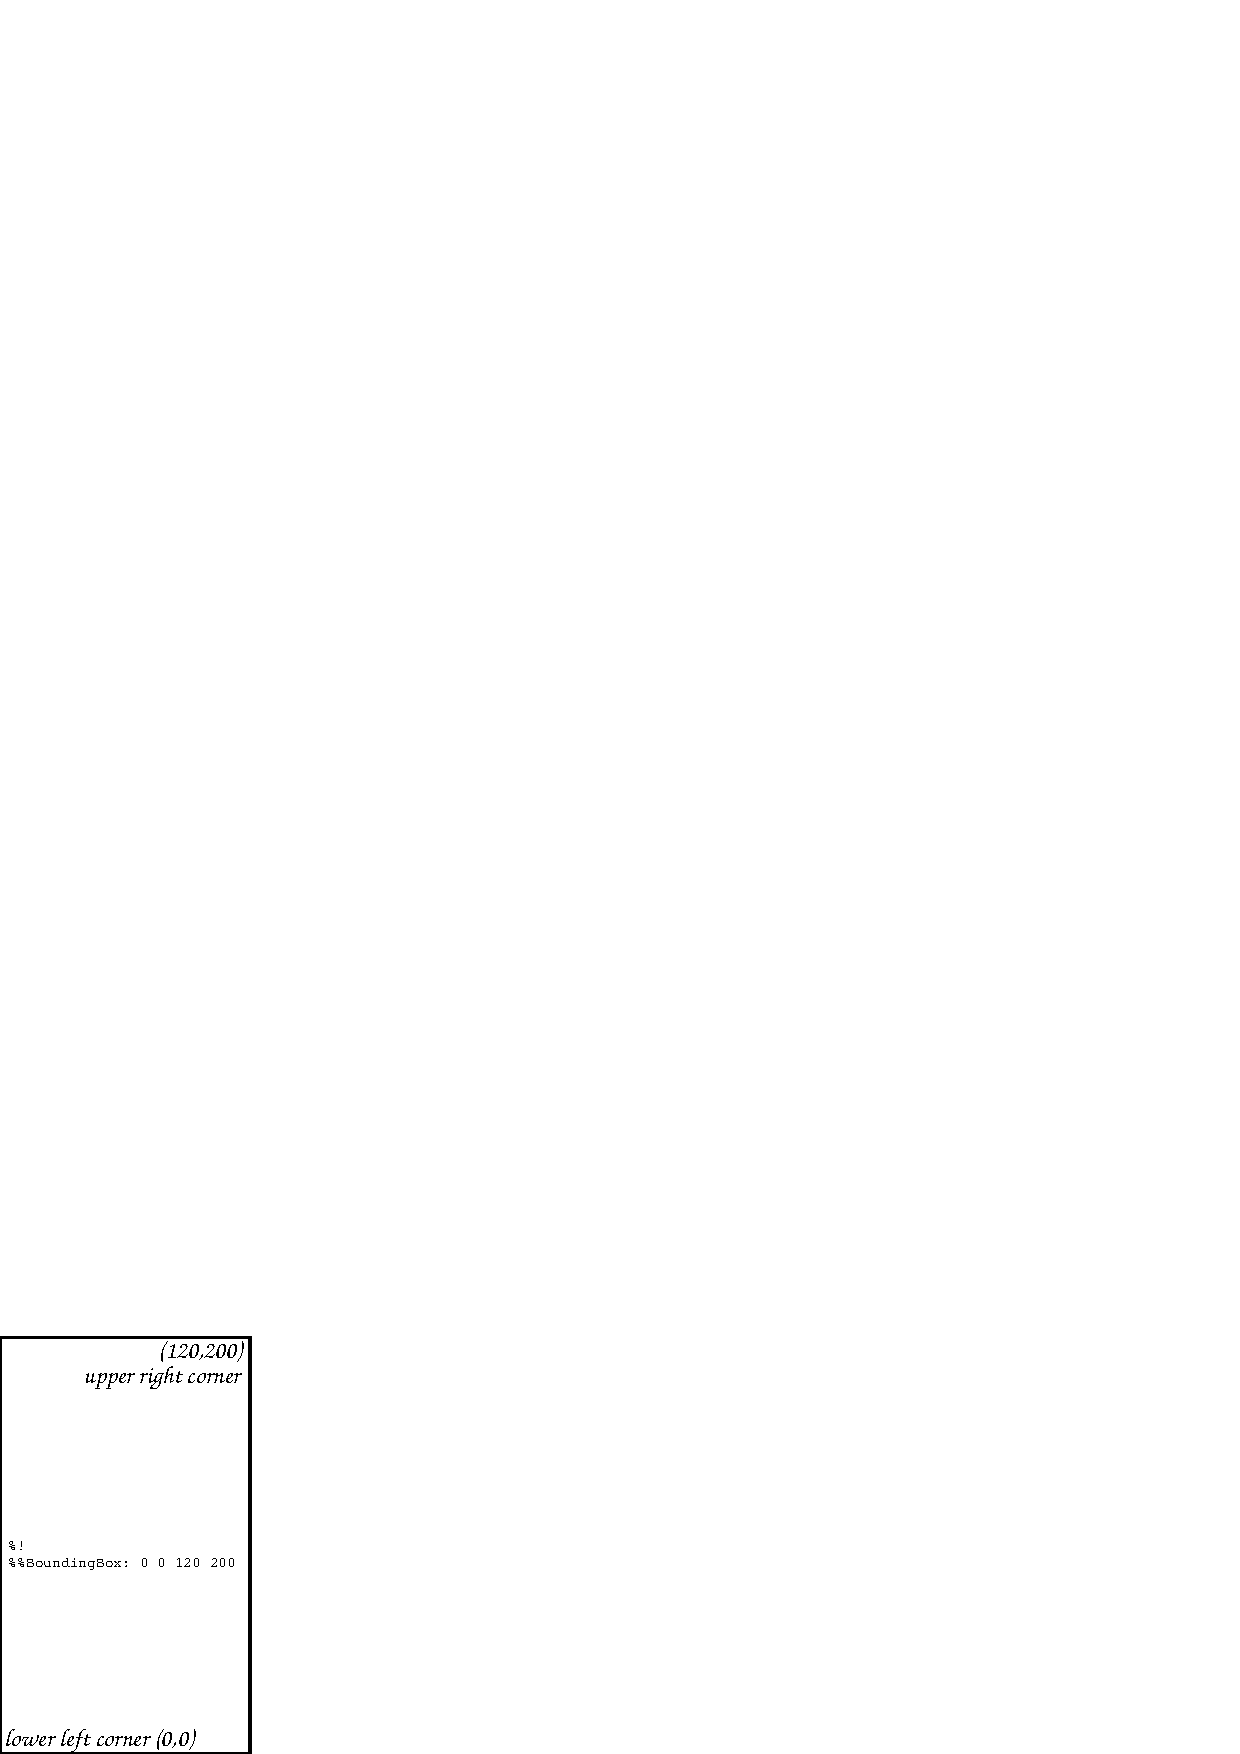
\includegraphics{fig1}
% \end{figure}


\end{document}                    % DO NOT DELETE THIS LINE
%%%%%%%%%%%%%%%%%%%%%%%%%%%%%%%%%%%%%%%%%%%%%%%%%%%%%%%%%%%%%%%%%%%%%%%%%%%%%%
